\NoBgThispage
\chapter{MapAlign: Deep-Learning based approach}

\section{Neural Networks}
Neural networks (NNs) are computational models inspired by the structure and functionality of the human brain, consisting of interconnected layers of neurons. Just as biological neurons process signals transmitted across synapses, artificial neurons in a neural network receive inputs, process them, and generate outputs \cite{Grosan2011}. These networks are primarily used in a wide range of machine learning tasks such as image recognition, natural language processing, and predictive analytics.
In this chapter the building blocks, main principles, and training methodologies of neural networks will be explored, starting with an in-depth discussion of the neuron as the basic unit.

\subsection{Neuron and its Function}
At the core of every neural network lies the artificial neuron, modeled after its biological counterpart. Each neuron receives input signals, which are processed and combined to produce an output. Mathematically, this process is represented as follows \cite{10.11648/j.ajnna.20190501.12}:
% Neuron Input
\begin{equation}
    \textit{net}_i = \sum_{j=1}^{d} w_{ji} \cdot \textit{in}_j + w_{0i}
\end{equation}

Here, $(\text{in}_1, \text{in}_2, \ldots, \text{in}_d)$ are the $d$ inputs the neuron receives, analogous to signals received by biological neurons through synapses. These inputs are weighted by $w_{ji}$, which are the synaptic weights, representing the strength of the connection between neurons, which can be either positive (if one unit excites another) or negative (if one unit suppresses or inhibits another). The higher the weight, the more influence one unit has on another. (This corresponds to the way actual brain cells trigger one another across tiny gaps called synapses) \cite{10.11648/j.ajnna.20190501.12}.

Learning in a neural network is essentially an adjustment of these weights. The term $w_{0i}$ is a bias that helps adjust the output and enhances the model's flexibility. The sum of these weighted inputs results in the neuron’s excitation level, denoted as $\textit{net}_i$.
Once the net input ${net}_i$ is computed, the neuron applies an activation function $f(\cdot)$ to determine the output:
% Neuron Output
\begin{equation}
    \textit{out}_i = f(\textit{net}_i)
\end{equation}

The activation function introduces non-linearity to the model, enabling neural networks to learn complex, non-linear mappings between inputs and outputs. Common activation functions include:
\begin{itemize}
    \item Sigmoid: Outputs values between $0$ and $1$.
    \item Tanh: Outputs values between $-1$ and $1$.
    \item ReLU: Outputs values following: $f(\textit{net}_i) = \max(0, \textit{net}_i)$.
\end{itemize}

\begin{figure}
    \centering
    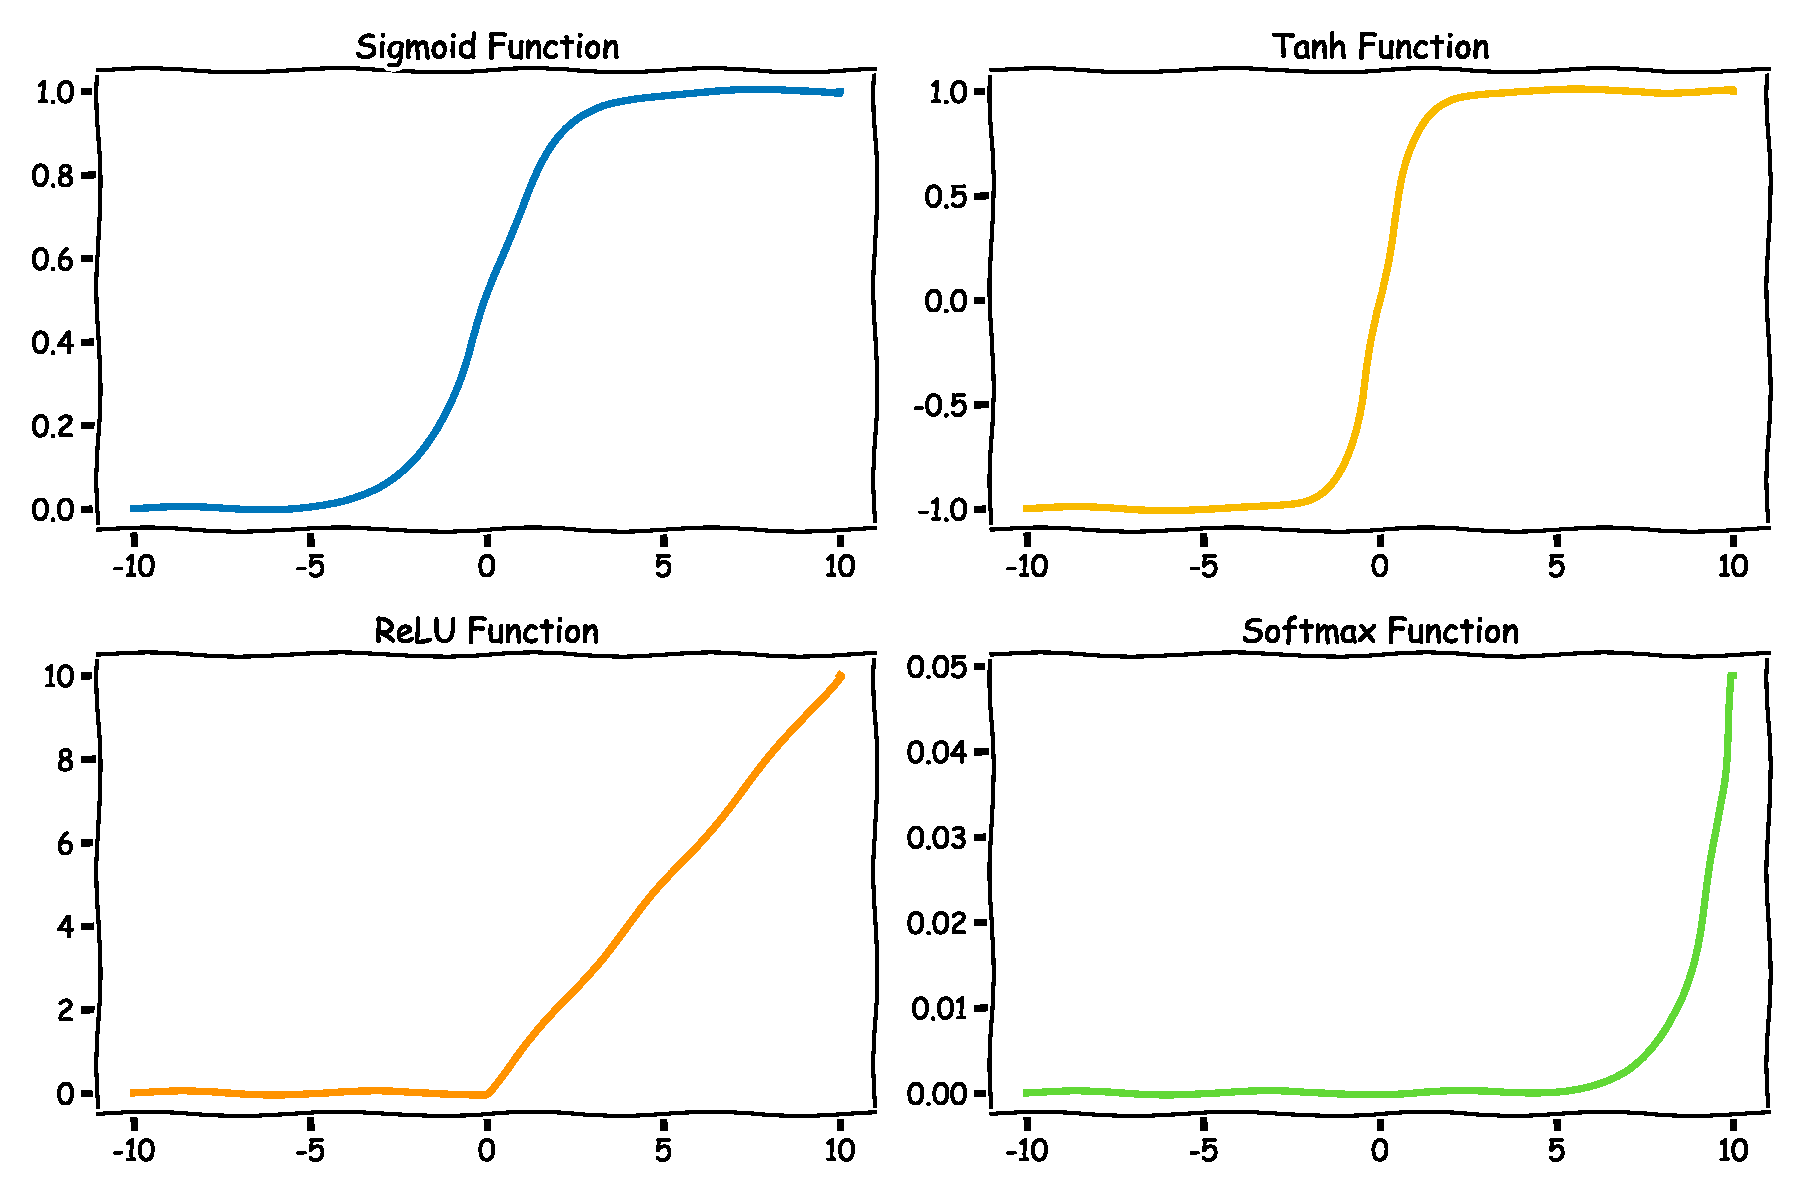
\includegraphics[width=1\linewidth]{LateX//figs/activation_functions_xkcd.pdf}
    \caption{Enter Caption}
    \label{fig:enter-label}
\end{figure}

In a neural network, the choice of activation function is critical, as it determines how data is transformed across the network layers. Among the various available activation functions, the Rectified Linear Unit (ReLU) is one of the most widely used due to its distinct advantages in training deep learning models.

ReLU is particularly popular because it introduces non-linearity without saturating for positive values, an issue that affects functions like Sigmoid and Tanh, which tend to have very small gradients at extreme values, leading to the vanishing gradient problem. Additionally, the simplicity of ReLU’s derivative allows for efficient back-propagation, enhancing computational speed during training and supporting convergence in deep networks.
% ReLU Derivative
\begin{equation}
    f'(\textit{net}_i) =
    \begin{cases}
    1, & \textit{net}_i > 0 \\
    0, & \textit{net}_i \leq 0
    \end{cases}
\end{equation}

Given the importance of ReLU and its advantageous properties, this function will be the focus in subsequent sections, as it will serve as the primary activation function in the architectures discussed.

\subsection{Neural Network Architecture}
Neural networks are generally organized in layers:
\begin{itemize}
    \item Input Layer: Takes in the raw data features.
    \item Output Layer: Outputs the final predictions.
    \item Hidden Layers: Contain intermediate neurons that extract hierarchical features. The presence of multiple hidden layers makes the network "deep," giving rise to deep neural networks (DNNs).
\end{itemize}

\begin{figure}
    \centering
    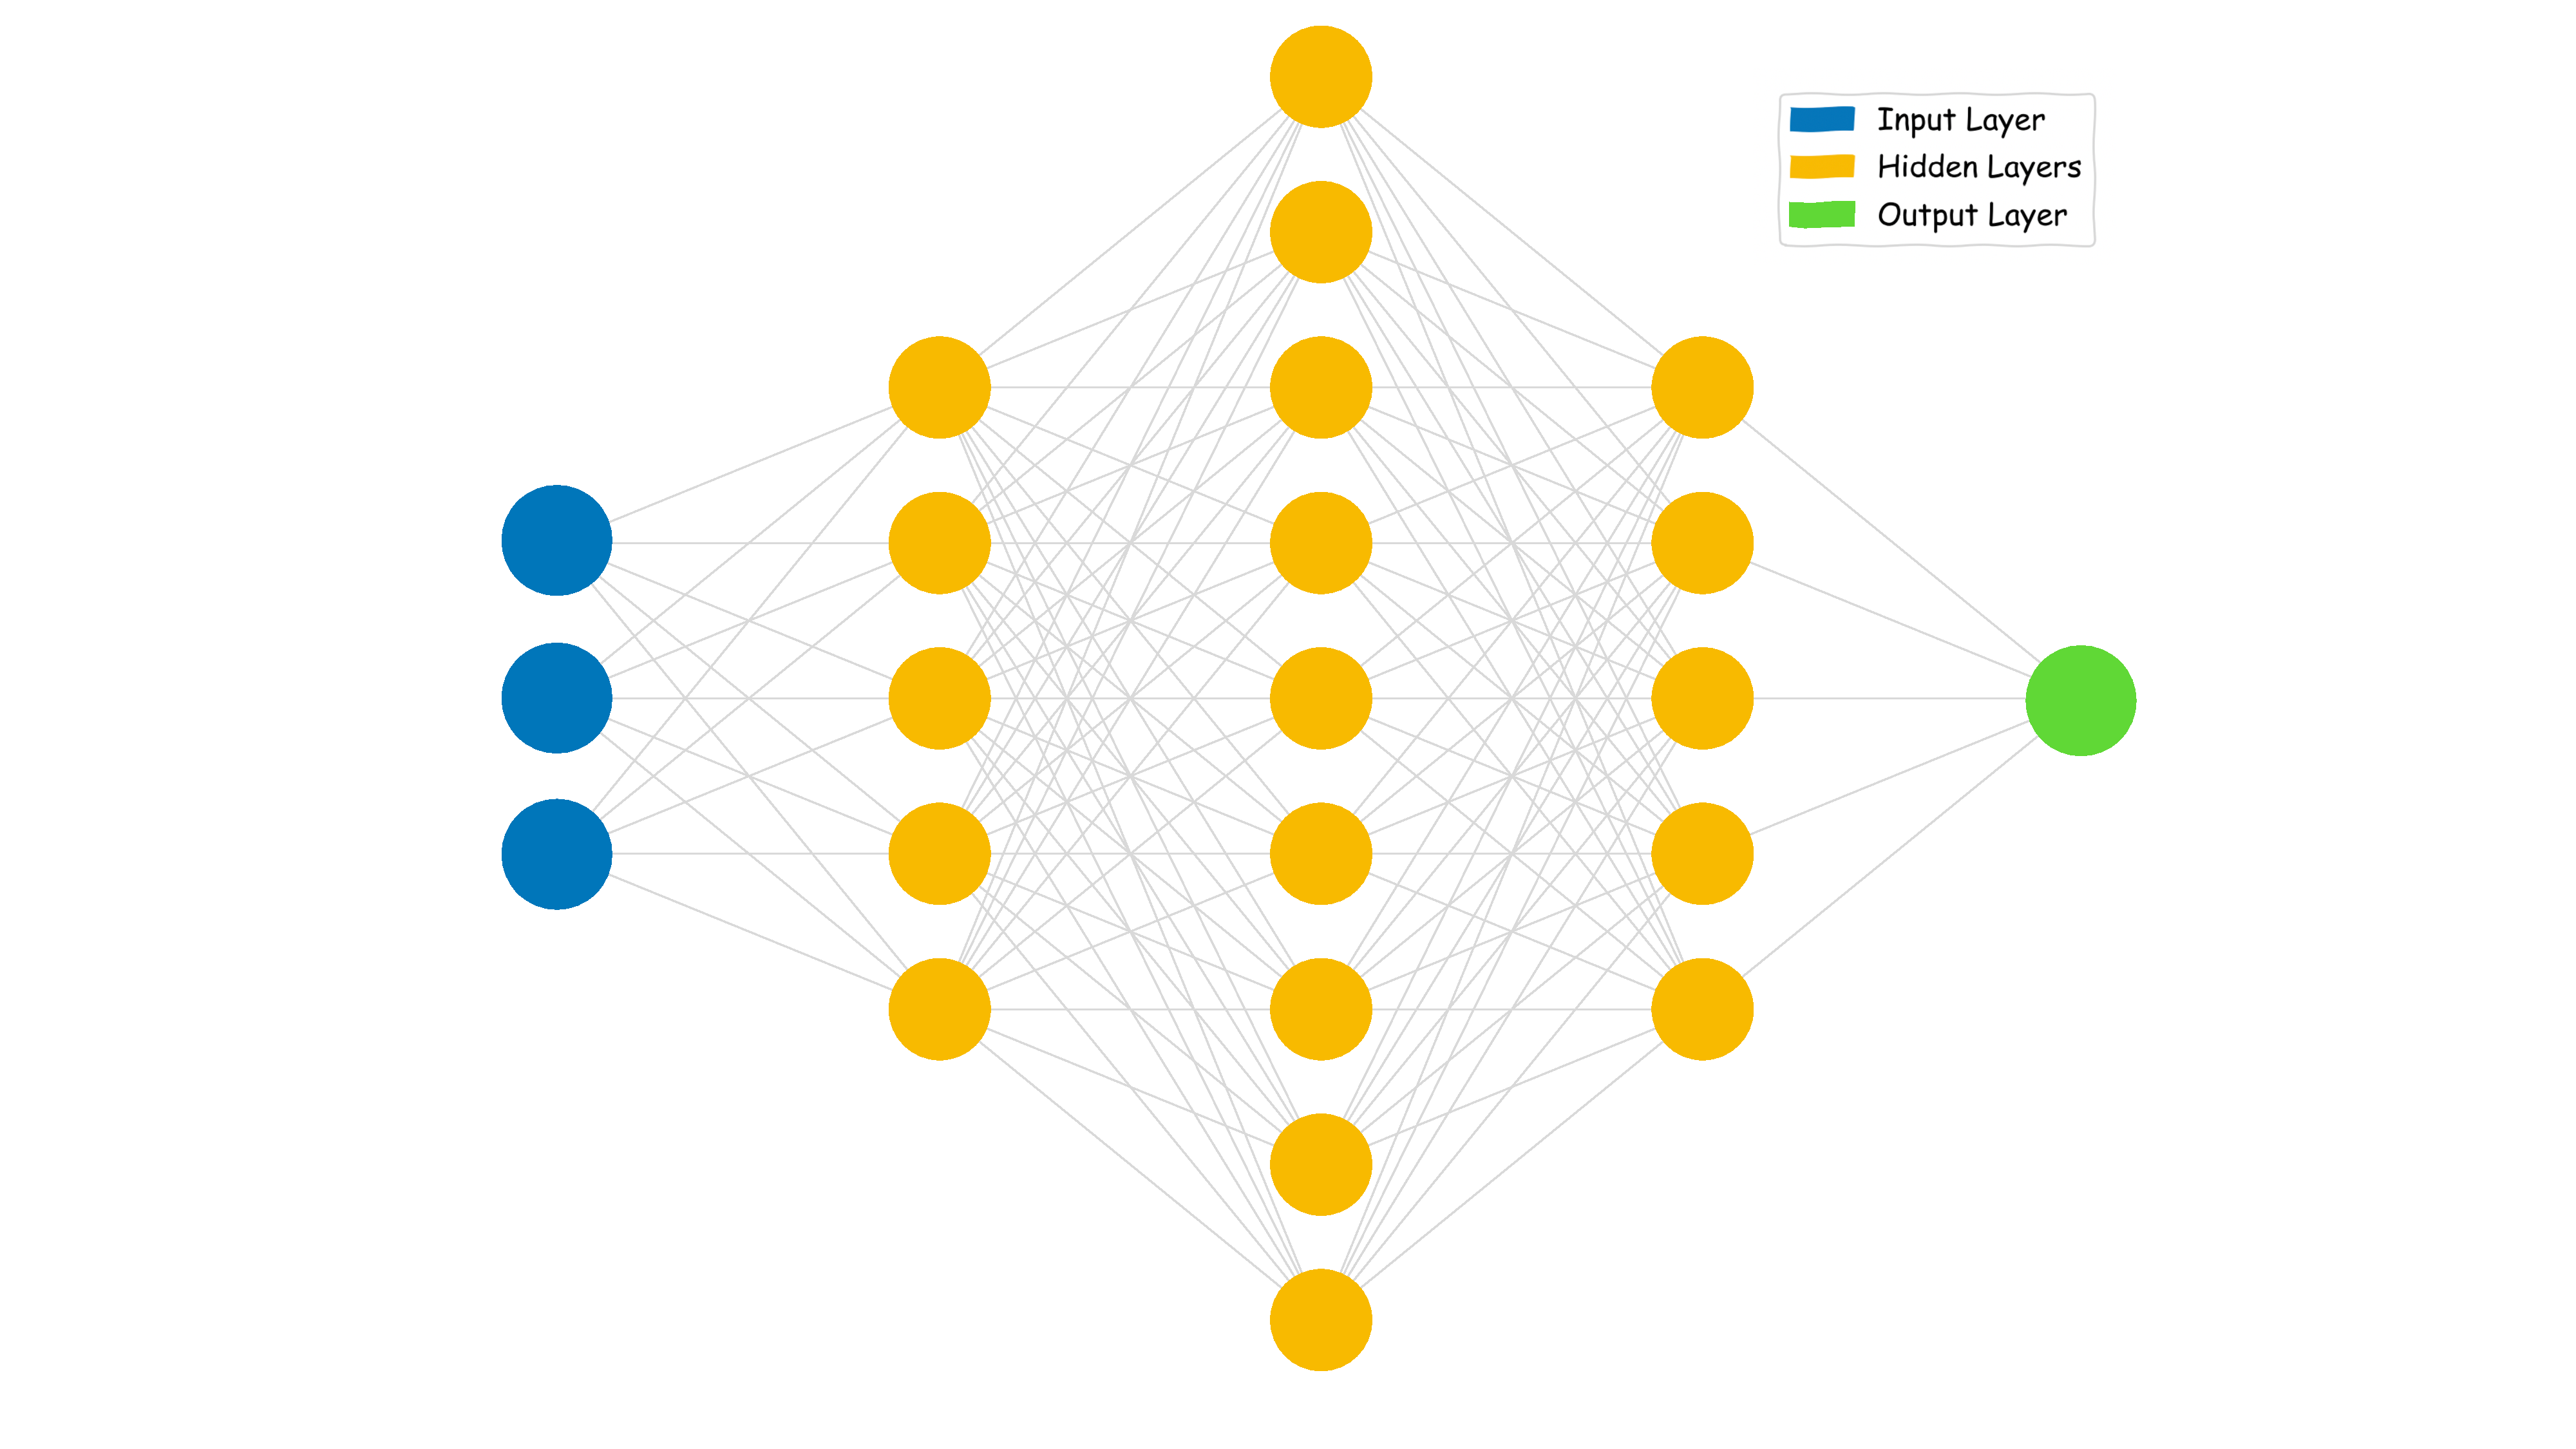
\includegraphics[width=0.9\linewidth]{LateX//figs/nn_intro_def.pdf}
    \caption{Enter Caption}
    \label{fig:enter-label}
\end{figure}

\subsubsection*{Forward Propagation}
Once the network architecture is defined, information propagates from the input layer to the output layer in a process called \textit{forward propagation}. This involves feeding inputs through each layer, applying the weights, summing them, and computing outputs using activation functions. The forward pass determines the final output for a given input.

\subsubsection*{Training Neural Networks}
The goal of training a neural network is to find the optimal set of weights $w_{ji}$ that map inputs to desired outputs. This process involves minimizing the difference between the network’s predictions and the actual targets, as measured by a \textit{loss function}.
Loss functions are a fundamental component of neural network training. They quantify the difference between the network's predictions and the true targets, guiding the network’s weight adjustments to reduce this difference. In essence, the loss function measures the "error" of the network's predictions, with the goal of minimizing this error to improve the network's accuracy.

Loss functions are a fundamental component of neural network training. They quantify the difference between the network's predictions and the true targets, guiding the network’s weight adjustments to reduce this difference. In essence, the loss function measures the "error" of the network's predictions, with the goal of minimizing this error to improve the network's accuracy.
The most common and widely used loss functions will be depicted in the following part:
\begin{itemize}
    \item \textbf{L1 Loss (Mean Absolute Error - MAE)}:  
    The L1 loss calculates the absolute difference between each predicted value and its corresponding true value. This function is also known as mean absolute error (MAE) and is defined as:
    \begin{equation}
        E(\mathbf{w}, \mathbf{x}) = \frac{1}{N} \sum_{i=1}^{N} |y_i - \hat{y}_i|
    \end{equation}
    where \( y_i \) is the true label, \( \hat{y}_i \) is the predicted output, and \( N \) is the number of data samples. L1 loss is robust to outliers because it does not square the error, which makes it less sensitive to large differences.

    \item \textbf{Smooth L1 Loss}:  
    The smooth L1 loss combines aspects of both L1 and L2 losses to make the loss function more robust to outliers but still sensitive to small errors. It is defined as:
    \begin{equation}
        E(\mathbf{w}, \mathbf{x}) = 
        \begin{cases} 
            0.5 \cdot (y_i - \hat{y}_i)^2 & \text{if } |y_i - \hat{y}_i| < 1 \\
          |y_i - \hat{y}_i| - 0.5 & \text{otherwise}
        \end{cases}
    \end{equation}

    Smooth L1 loss is particularly useful in regression tasks where outliers might be present but penalizing large errors less than quadratic losses is still desirable.

    \item \textbf{Mean Squared Error (MSE)}:  
    Mean squared error, also known as L2 loss, calculates the average of the squared differences between predicted and actual values:
    \begin{equation}
        E(\mathbf{w}, \mathbf{x}) = \frac{1}{N} \sum_{i=1}^{N} (y_i - \hat{y}_i)^2
    \end{equation}
   
    Squaring the errors makes the MSE more sensitive to larger errors, which can be beneficial in some cases but can lead to instability if outliers are present.

    \item \textbf{Sum of Squared Errors (SSE)}:  
    A variation of MSE, the sum of squared errors (SSE) measures the total squared difference between predicted and actual values, without averaging over the number of samples:
    \begin{equation}
        E(\mathbf{w}, \mathbf{x}) = \frac{1}{2} \sum_{i=1}^{N} (y_i - \hat{y}_i)^2
    \end{equation}
    
    SSE is widely used in gradient-based optimization, particularly because of its mathematical properties that simplify gradient calculations. Dividing by 2 is standard, as it cancels out the exponent when differentiating with respect to the weights.
\end{itemize}

Each of these loss functions offers unique benefits, with L1 and smooth L1 loss being more robust to outliers, while MSE and SSE penalize larger errors more heavily. Choosing the right loss function is critical and should be based on the specifics of the task and the characteristics of the data.

\begin{figure}[H]
    \centering
    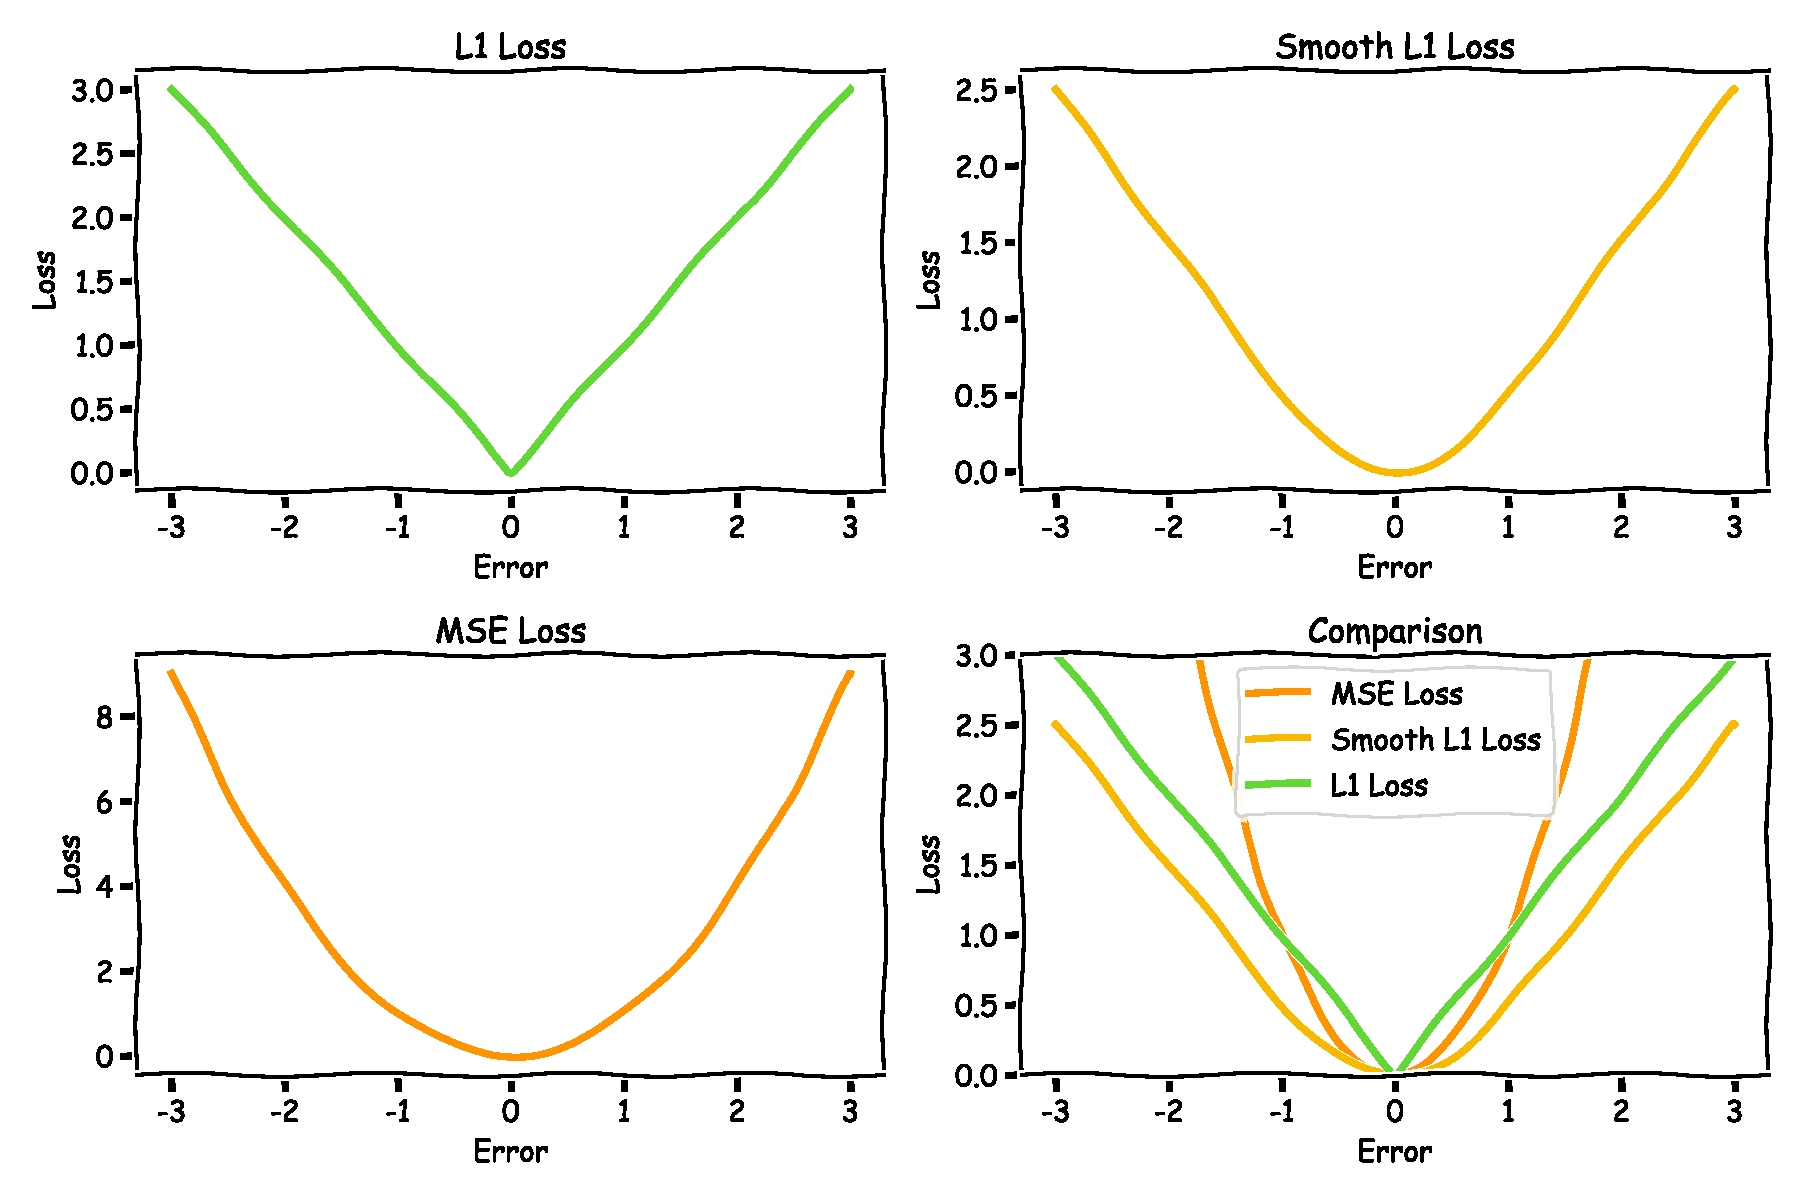
\includegraphics[width=1\linewidth]{LateX/figs/loss_functions_xkcd.pdf}
    \caption{Enter Caption}
    \label{fig:enter-label}
\end{figure}

\subsubsection*{Gradient Descent and Back-propagation}
To minimize the loss function, neural networks use the gradient descent algorithm, which updates the weights by moving them in the direction opposite to the gradient of the loss function. 
\begin{equation}
    \nabla_\theta L = \frac{\partial L}{\partial \theta}
\end{equation}

In neural networks, after computing the gradients via back-propagation, the following step is to update the weights to minimize the loss function. This is done using an optimizer, which controls how the weights are adjusted based on the gradients. The learning rate $\eta$ is a key hyper-parameter in this update process, determining the step size in the direction of the gradient. 
A proper learning rate is crucial: if it's too large, the network may overshoot the optimal solution; if it's too small, convergence becomes slow and inefficient.
\begin{figure}[H]
    \centering
    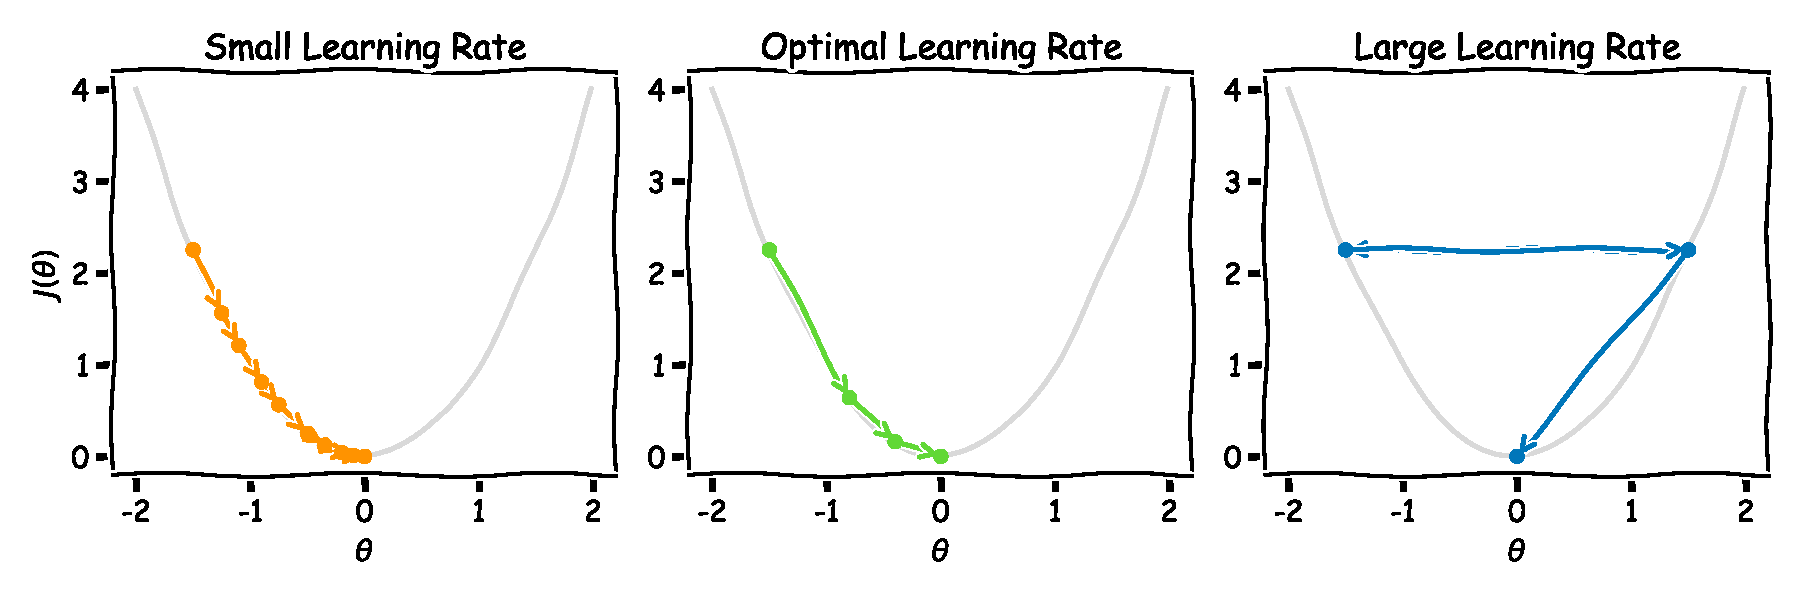
\includegraphics[width=1\linewidth]{LateX//figs/learning_rate.pdf}
    \caption{Enter Caption}
    \label{fig:enter-label}
\end{figure}

The optimizer updates the weights accordingly the following general rule:
\begin{equation}
    \theta \leftarrow \theta - \eta \nabla_\theta L
\end{equation}
where where: $\theta$ represents the weights, $\eta$ depicts the learning rate and $\nabla L_\theta$ is the gradient of the loss function with respect to the weights. 

Two of the most commonly used optimizers are Stochastic Gradient Descent (SGD) and Adam.

\subsubsection*{Stochastic Gradient Descent}
A practical variant of gradient descent, especially for large datasets, is stochastic gradient descent (SGD). Unlike traditional gradient descent, which computes the gradient over the entire dataset, SGD computes the gradient for a subset of the data, known as a mini-batch, and updates the weights after each \textit{mini-batch}. This introduces a level of randomness into the process but has the advantage of significantly speeding up training, especially when working with large datasets. SGD is more likely to escape \textit{local minima} and can result in better generalization.

\begin{algorithm}
\caption{Stochastic Gradient Descent (SGD)}
\begin{algorithmic}[1]
\State \textbf{Initialize:} weights $\theta_{ih}, \theta_{ho}, \eta$, batch size $B$, max epochs $T_{\text{max}}$
\State $t \gets 0$

\Repeat
    \State $t \gets t + 1$
    \State $L \gets 0$ \Comment{Initialize loss}
    \State Randomly shuffle the training set $\mathcal{D}$

    \For {each mini-batch $\mathcal{B}$ of size $B$}
        \State Reset gradient: $\nabla \theta_{ih} \gets 0, \nabla \theta_{ho} \gets 0$
        
        \For {each sample $x_i$ in $\mathcal{B}$}
            \State \textbf{Forward step:} $y_i \gets \text{forward}(x_i, \theta_{ih}, \theta_{ho})$
            \State Compute loss $L \gets L + \mathcal{L}(y_i, t_i)$
            
            \State \textbf{Backward step:} Compute gradients $\nabla \theta_{ho}, \nabla \theta_{ih}$ 
        \EndFor

        \State Update hidden-output weights: $\theta_{ho} \gets \theta_{ho} - \eta \cdot \nabla \theta_{ho}$
        \State Update input-hidden weights: $\theta_{ih} \gets \theta_{ih} - \eta \cdot \nabla \theta_{ih}$
        
        \State $L \gets L / B$ \Comment{Average the loss}
    \EndFor
    
\Until {(not convergence \textbf{and} $t < T_{\text{max}}$)}

\end{algorithmic}
\end{algorithm}

Another popular optimizer, especially in deep learning, is the Adam (short for Adaptive Moment Estimation) optimizer. Adam combines the benefits of both momentum and adaptive learning rates. It calculates individual adaptive learning rates for each parameter by considering both the first moment (the mean) and the second moment (the uncentered variance) of the gradients.
\begin{equation}
    \theta_t = \theta_{t-1} - \eta \cdot \frac{\hat{m}_t}{\sqrt{\hat{v}_t} + \epsilon}
\end{equation}
In the formula: \(\theta_t\) is the updated weight, \(\theta_{t-1}\) is the previous weight, \(\eta\) is the learning rate, \(\hat{m}_t\) is the bias-corrected first moment estimate, \(\hat{v}_t\) is the bias-corrected second moment estimate, and \(\epsilon\) is a small constant to prevent division by zero.

\begin{algorithm}
\caption{Adam Optimizer}
\begin{algorithmic}[1]
\State \textbf{Initialize:} weights \(\theta_{ih}, \theta_{ho}, \eta\), batch size \(B\), max epochs \(T_{\text{max}}\), \(\beta_1, \beta_2\), \(\epsilon\)
\State \(m_{ih} \gets 0, v_{ih} \gets 0, m_{ho} \gets 0, v_{ho} \gets 0\) \Comment{Initialize parameters}
\State \(t \gets 0\) \Comment{Initialize time-step}

\Repeat
    \State \(t \gets t + 1\)
    \State \(L \gets 0\) \Comment{Initialize loss}
    \State Randomly shuffle the training set \(\mathcal{D}\)

    \For {each mini-batch \(\mathcal{B}\) of size \(B\)}
        \State Reset gradients: \(\nabla \theta_{ih} \gets 0, \nabla \theta_{ho} \gets 0\)

        \For {each sample \(x_i\) in \(\mathcal{B}\)}
            \State \textbf{Forward step:} \(y_i \gets \text{forward}(x_i, \theta_{ih}, \theta_{ho})\)
            \State Compute loss \(L \gets L + \mathcal{L}(y_i, t_i)\)

            \State \textbf{Backward step:} Compute gradients \(\nabla \theta_{ho}, \nabla \theta_{ih}\)
        \EndFor

        \State Update first moment estimates: 
        \[
        m_{ih} \gets \beta_1 \cdot m_{ih} + (1 - \beta_1) \cdot \nabla \theta_{ih}, \quad m_{ho} \gets \beta_1 \cdot m_{ho} + (1 - \beta_1) \cdot \nabla \theta_{ho}
        \]
        \State Update second moment estimates: 
        \[
        v_{ih} \gets \beta_2 \cdot v_{ih} + (1 - \beta_2) \cdot (\nabla \theta_{ih})^2, \quad v_{ho} \gets \beta_2 \cdot v_{ho} + (1 - \beta_2) \cdot (\nabla \theta_{ho})^2
        \]
        \State Bias correction:
        \[
        \hat{m}_{ih} \gets \frac{m_{ih}}{1 - \beta_1^t}, \quad \hat{m}_{ho} \gets \frac{m_{ho}}{1 - \beta_1^t}
        \]
        \[
        \hat{v}_{ih} \gets \frac{v_{ih}}{1 - \beta_2^t}, \quad \hat{v}_{ho} \gets \frac{v_{ho}}{1 - \beta_2^t}
        \]

        \State Update weights: 
        \[
        \theta_{ih} \gets \theta_{ih} - \eta \cdot \frac{\hat{m}_{ih}}{\sqrt{\hat{v}_{ih}} + \epsilon}
        \]
        \[
        \theta_{ho} \gets \theta_{ho} - \eta \cdot \frac{\hat{m}_{ho}}{\sqrt{\hat{v}_{ho}} + \epsilon}
        \]

        \State \(L \gets L / B\) \Comment{Average the loss}
    \EndFor

\Until {(not convergence \textbf{and} \(t < T_{\text{max}}\))}

\end{algorithmic}
\end{algorithm}

In this section, we have introduced the fundamental structure of neural networks, focusing on their building blocks, including neurons, layers, and connections. We have discussed the forward pass, where inputs are processed through hidden layers to produce an output, and the back-propagation process used to adjust the weights based on the error calculated at the output.

The following steps outline the typical workflow for training a neural network using back-propagation \cite{10.11648/j.ajnna.20190501.12}:

\begin{enumerate} 
    \item Assign random weights to all the linkages to initialize the network. 
    \item Using the inputs and the linkages from Input to Hidden Nodes, compute the activation of Hidden Nodes. 
    \item Using the activation of Hidden Nodes and the linkages to Output Nodes, compute the activation of Output Nodes. 
    \item Calculate the error at the output node by comparing the predicted and actual outputs. 
    \item Propagate the error back through the network, adjusting the weights between the Output Nodes and the Hidden Nodes. 
    \item Using the error at the Output node, propagate the error back to the Hidden Nodes and adjust the weights between the Hidden and Input Nodes. 
    \item Repeat the process iteratively, adjusting the weights until the convergence criterion is met (e.g., minimal error or a maximum number of epochs). 
    \item Once trained, use the final weights to make predictions by scoring the activation rate of the Output Nodes. 
\end{enumerate}

This iterative process, combined with optimization techniques such as gradient descent, allows neural networks to learn from data and improve over time. In the following chapters, we will explore how these principles are applied to more complex architectures and tasks, including their use in localization methods for autonomous driving.

\subsection{Convolutional Neural Network (CNN)}

A Convolutional Neural Network (CNN), or \textit{ConvNet}, is a specialized type of deep learning algorithm primarily designed for tasks requiring object recognition, such as image classification, detection, and segmentation. CNNs are widely employed in various practical applications, ranging from autonomous vehicles and medical imaging to security camera systems and facial recognition technologies \cite{DBLP:journals/corr/OSheaN15}. CNNs are architecturally distinct from traditional neural networks, as they take into account the spatial structure of data—usually images—by arranging neurons in a way that mimics the human visual cortex. The network's architecture is typically organized in layers, including convolutional layers\footnote{A convolutional layer is responsible for applying a set of filters (kernels) to the input image, producing feature maps that highlight important patterns like edges, textures, or shapes.}, pooling layers\footnote{A pooling layer reduces the spatial dimensions of the feature maps, typically by using operations like max pooling or average pooling, which helps reduce computational load and control over-fitting.}, and fully connected layers\footnote{Fully connected layers are the traditional neural network layers where every neuron is connected to every neuron in the previous layer. They typically occur at the end of the network and help in decision-making, such as classifying an image into categories.}, each playing a pivotal role in feature extraction and decision making.

Convolutional Neural Networks (CNNs) are specifically designed to process 2D data, such as images, more efficiently than fully connected networks by utilizing convolutional operations instead of traditional matrix multiplications. This architecture enables CNNs to capture spatial hierarchies of patterns in image data, from low-level edges to high-level features like objects or faces.

The basic building blocks of CNNs include:

\begin{enumerate}
    \item \textbf{Convolutional Layers}: These layers apply convolutional operations to the input data. In mathematical terms, a convolution operation is defined as:
    \begin{equation}
        (f * g)(x, y) = \sum_{m}\sum_{n}f(m, n) \cdot g(x - m, y - n)
    \end{equation}
    \begin{figure}[H]
        \centering
        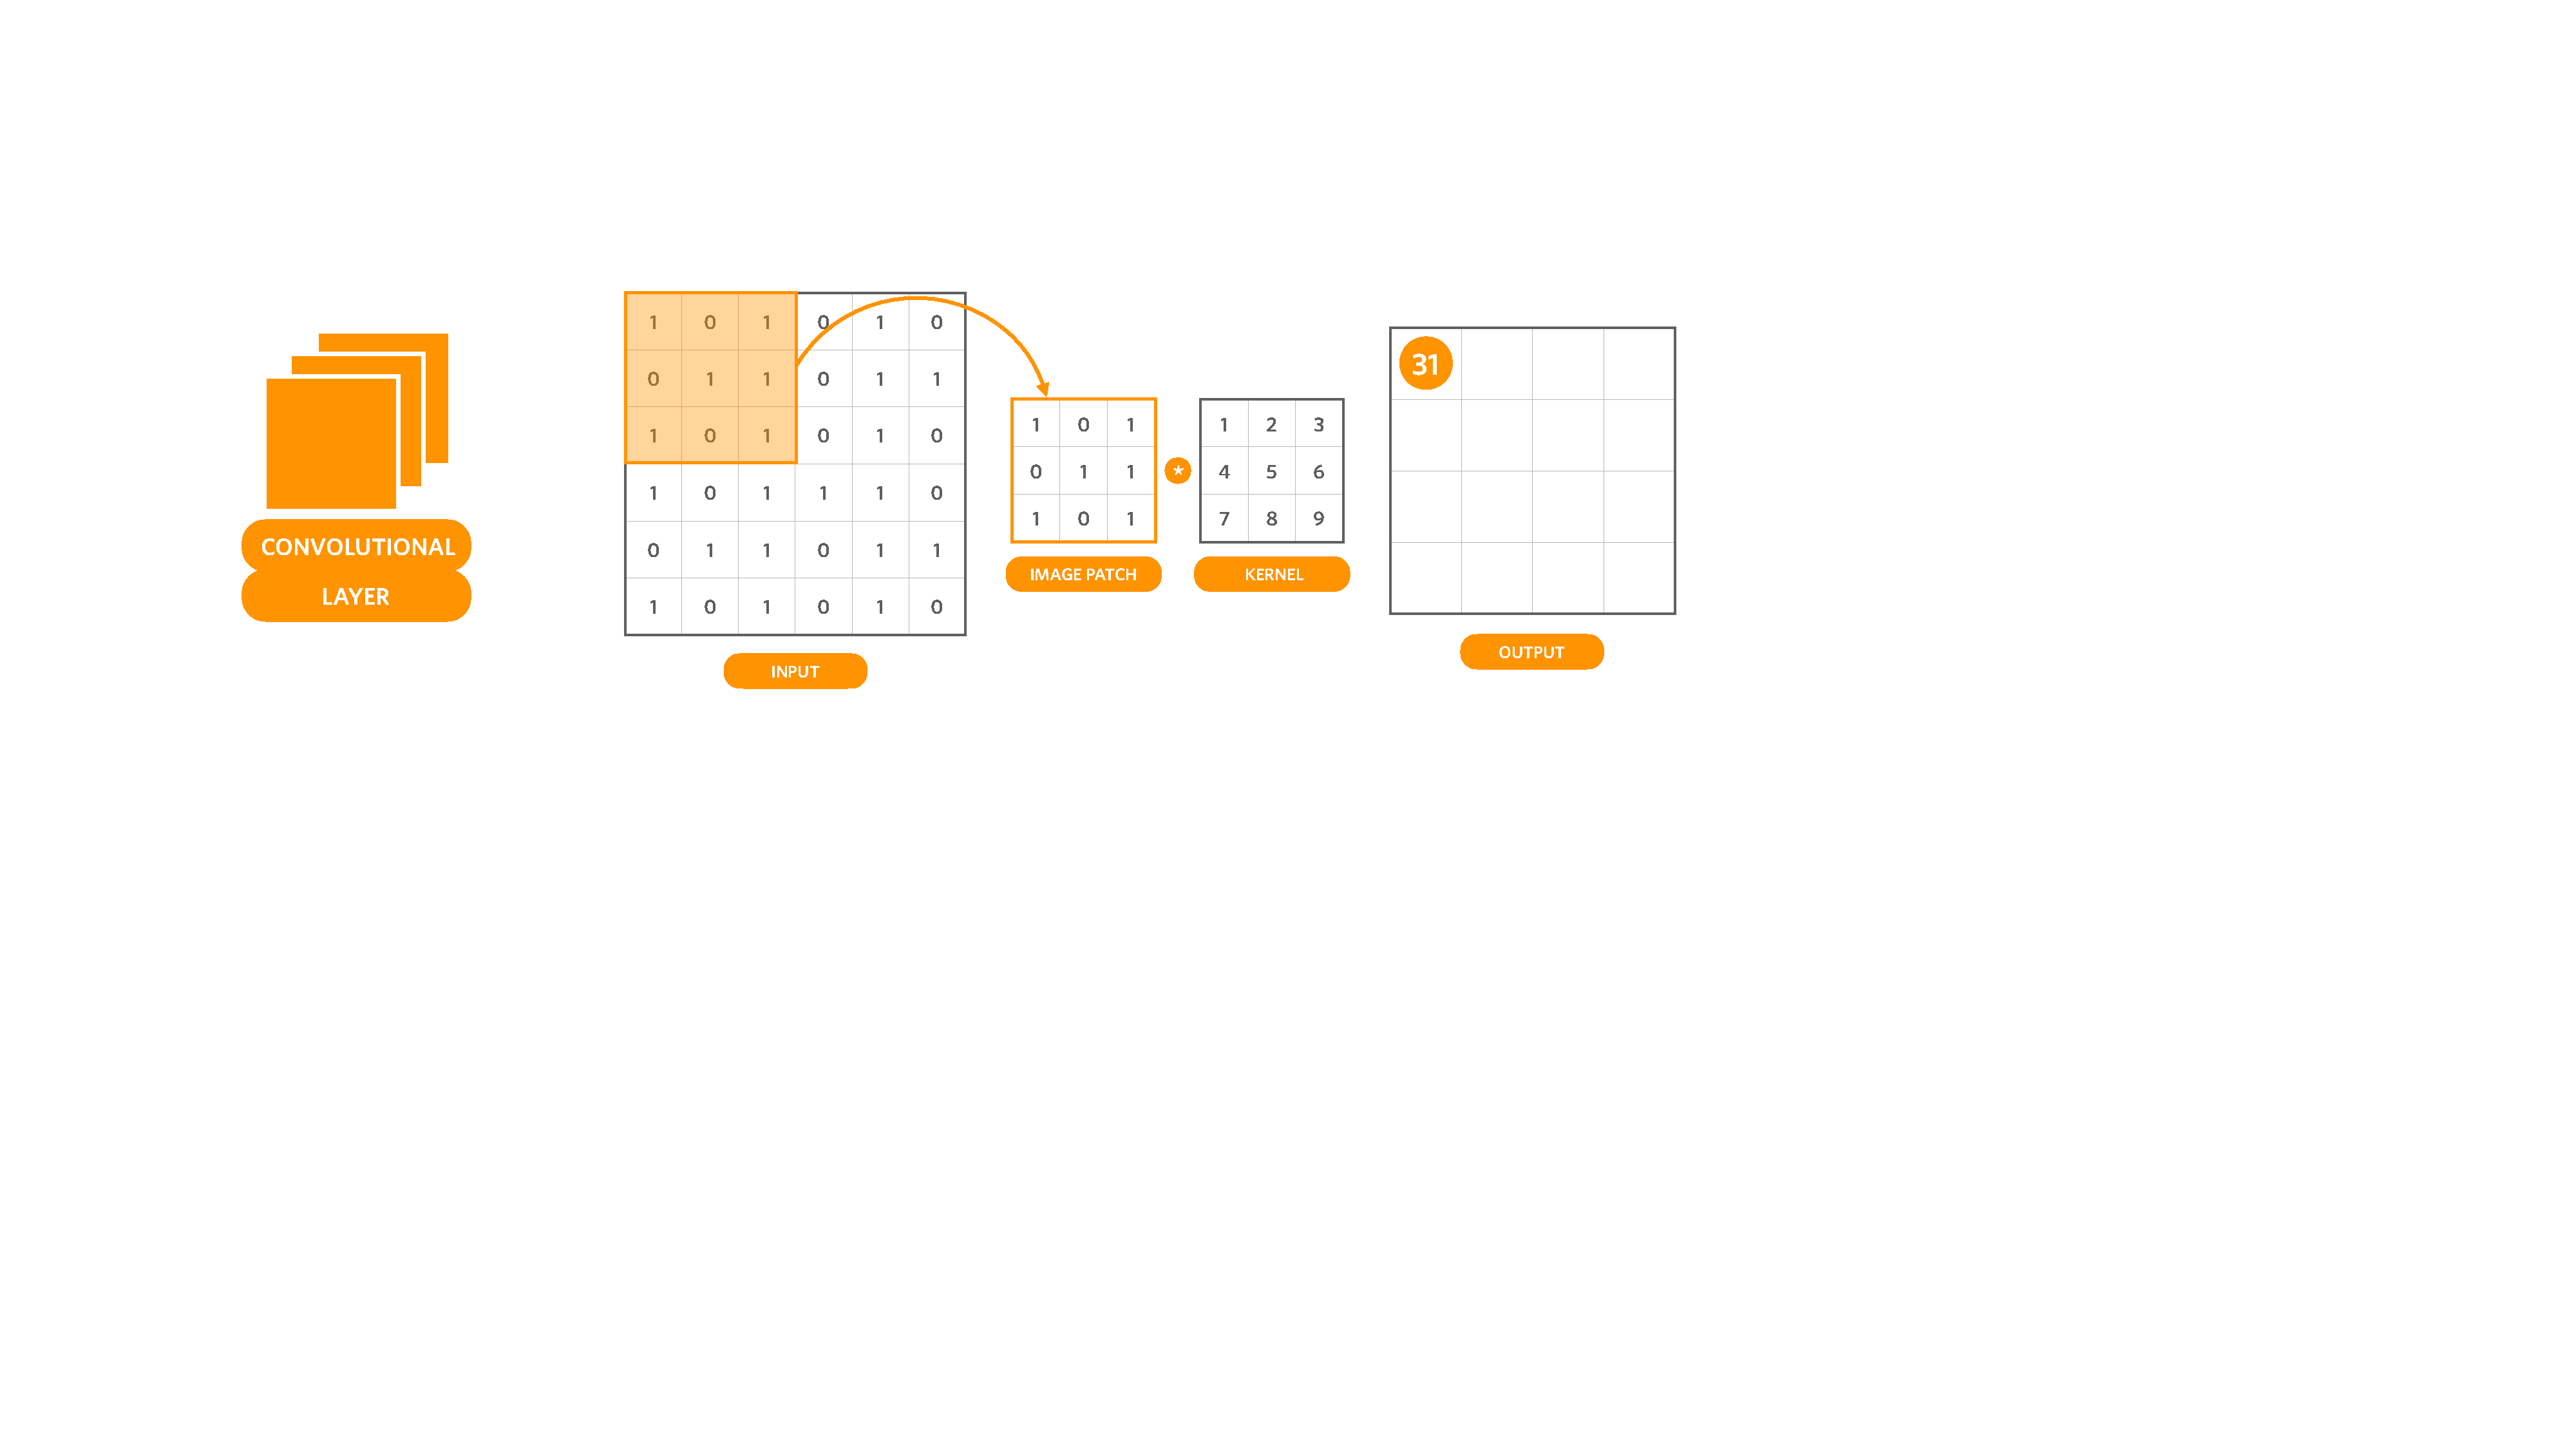
\includegraphics[width=1\linewidth]{LateX//figs/CCN_layer.pdf}
        \caption{Enter Caption}
        \label{fig:enter-label}
    \end{figure}
    where \( f \) represents the input and \( g \) denotes the kernel (or filter). For a 2D image, the convolution operation involves sliding a filter over the input image and computing the dot product between the filter and segments of the image, resulting in an \textit{activation map}. The kernels are learnable parameters, allowing the CNN to automatically learn feature detectors for edges, textures, and more complex patterns. Each filter responds to a particular feature within the input, such as vertical edges or textures.

    \item \textbf{Rectified Linear Unit (ReLU)}: ReLU applies a non-linear transformation element-wise after the convolution operation. Its mathematical formulation is simple and it is already mentioned in above sections.

    \item \textbf{Pooling Layers}: Pooling layers reduce the spatial dimensions of activation maps while preserving important information. The most common form is max pooling, which selects the maximum value from each patch of the feature map. The formula for max pooling is:
    \begin{equation}
        P = \max_{(i,j) \in \text{patch}} x(i,j)
    \end{equation}
    \begin{figure}[H]
        \centering
        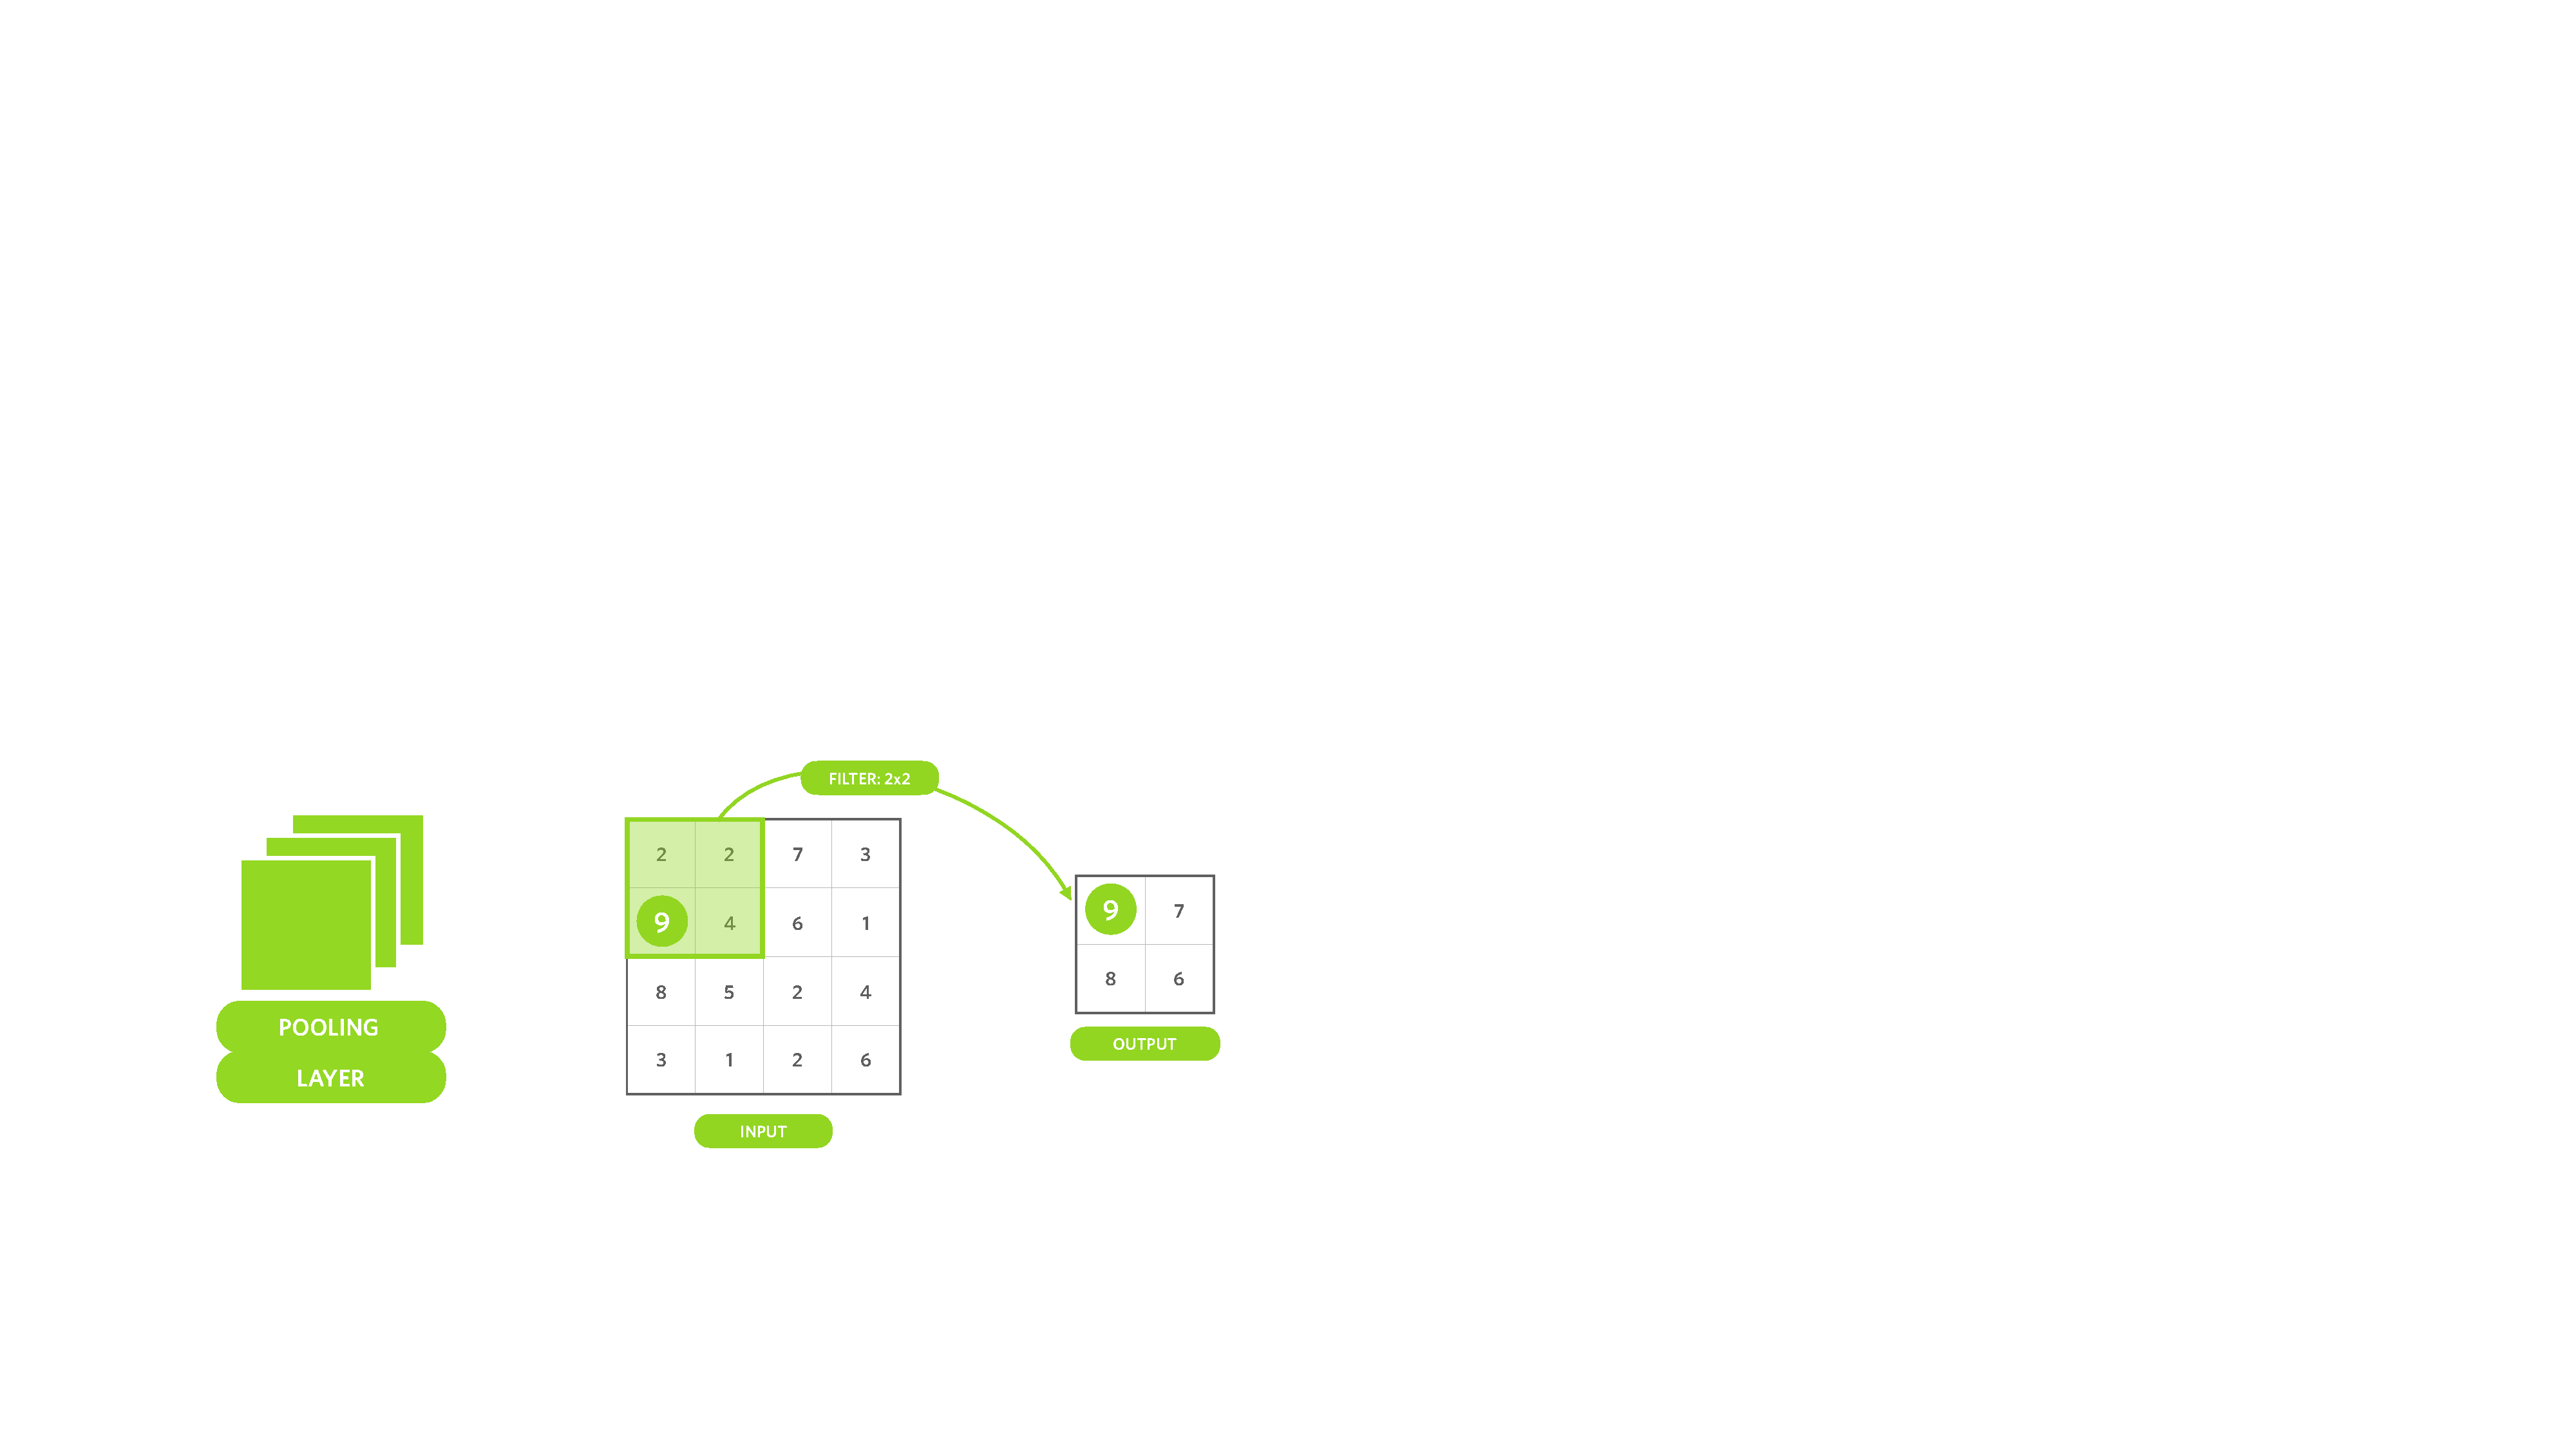
\includegraphics[width=0.85\linewidth]{LateX//figs/CNN_poolinh.pdf}
        \caption{Enter Caption}
        \label{fig:enter-label}
    \end{figure}
    where \( P \) is the pooling window, and \( x(i,j) \) represents values within this window. Pooling contributes to translation invariance, making the network more robust to variations in the input's position or scale.

    \item \textbf{Fully Connected Layers}: In the final layers of a CNN, fully connected layers perform the actual classification task. These layers take the high-level features detected by previous layers and map them to the final output, such as class probabilities in image classification tasks. This is where the network "decides" based on the features it has learned through previous layers.
\end{enumerate}

One of the key advantages of Convolutional Neural Networks (CNNs) over traditional machine learning models, such as Support Vector Machines (SVMs) or Decision Trees, is their ability to automatically learn features. Unlike traditional models that require manual feature extraction, CNNs autonomously learn hierarchical representations of data by employing multiple convolutional and pooling layers to extract features at various levels of abstraction.

CNNs are also commonly used as \textit{feature extractors} or \textit{backbones} in more complex neural network architectures. Their ability to automatically learn and generalize hierarchical features enables them to serve as powerful foundational networks that facilitate advanced tasks in various domains.

The main advantages of CNNs include:
\begin{itemize}
    \item \textbf{Translation Invariance}: CNNs achieve translation invariance by applying the same convolutional filters across different parts of the image. This enables the network to recognize objects even when they appear in different locations within the image, which is a substantial advantage over traditional methods that often require manually engineered features.

    \item \textbf{Hierarchical Feature Learning}: CNNs detect features in a hierarchical manner. In the initial layers, they capture low-level features such as edges, corners, or textures. In deeper layers, they detect higher-level, abstract features like shapes or object parts. This hierarchical learning process is akin to how the human visual cortex processes visual stimuli, progressing from simple to complex patterns.

    \item \textbf{Efficiency}: By using local connectivity, each neuron in convolutional layers is connected only to a small region of the input, known as the \textit{receptive field}, rather than the entire input. This significantly reduces computational requirements. Additionally, weight sharing in convolution layers, where the same filter is applied across different regions, reduces the number of parameters compared to fully connected networks, making CNNs computationally efficient.
\end{itemize}

Over time, various CNN architectures have been developed to optimize performance for specific tasks. Notable architectures include:
\begin{enumerate}
    \item \textbf{VGG-16}: Known for its simplicity, VGG-16 uses small \(3 \times 3\) convolutional filters but stacks a large number of convolutional layers followed by fully connected layers, creating a deep architecture with strong feature extraction capabilities \cite{7486599}.

    \item \textbf{ResNet}: ResNet introduced the concept of residual learning, which enables the training of very deep architectures. By incorporating skip connections, ResNet addresses the vanishing gradient problem, allowing for efficient training of deep networks. Various versions of ResNet exist, distinguished by the number of layers they contain, such as ResNet-18, ResNet-34, ResNet-50, ResNet-101, and ResNet-152. The number indicates the total layers, with deeper variants like ResNet-101 and ResNet-152 providing increasingly refined feature representations while maintaining efficient training \cite{DBLP:journals/corr/HeZRS15, 10197463}.

    \item \textbf{Inception (GoogLeNet)}: The Inception network incorporates convolutional layers of varying sizes applied in parallel. This multi-scale approach allows the network to capture features at different levels of granularity, enhancing its ability to recognize complex patterns \cite{DBLP:journals/corr/SzegedyLJSRAEVR14}.

    \item \textbf{EfficientNet}: This model family scales network width, depth, and resolution to achieve higher accuracy with fewer parameters. EfficientNet strikes a balance between accuracy and efficiency, making it a popular choice for many practical applications \cite{DBLP:journals/corr/abs-1905-11946}.
\end{enumerate}

While CNNs were originally designed for image-related tasks, their versatility has led to adaptations in various other domains, including:
\begin{itemize}
    \item \textbf{Natural Language Processing (NLP)}: CNNs are used for tasks such as text classification by applying convolutional filters over word embeddings, allowing the network to capture local dependencies in textual data.

    \item \textbf{Time Series Analysis}: CNNs can be applied to temporal data, effectively capturing local dependencies between data points over time, making them suitable for analyzing patterns in time series data.

    \item \textbf{Speech Recognition}: In combination with Recurrent Neural Networks (RNNs) or Transformers, CNNs can be utilized in speech recognition tasks, such as voice recognition or speech-to-text conversion, where they contribute to feature extraction and processing.
\end{itemize}

Through these applications, CNNs have proven to be a flexible and powerful tool in both traditional and emerging fields, providing a foundation for extracting robust features that can enhance the performance of complex neural networks.

\subsection{Transformers}


\section{MapAlign: Architecture description}
This section introduces MapAlign, the neural network developed in this thesis, following an initial overview of neural networks. The purpose of MapAlign is to integrate seamlessly into the pipeline of RTMG, a neural network introduced in (INSERIRE CAPITOLO) that is able to generate HD maps in real time. 
MapAlign would be positioned in the pipeline specifically at the dataset creation stage, where it addresses a crucial requirement for RTMG: achieving perfect alignment between data from the vehicle's sensor suite and the HD map, which serves as the RTMG network’s target.
One of MapAlign’s key contributions is automating the creation of ground-truth data by significantly reducing the need for traditional optimization methods and, most importantly, by removing the necessity for manual alignment, a step previously required to ensure data precision. This integration allows the entire system to operate with greater autonomy, enabling faster and more reliable dataset creation. 
The objective of the model is to output values to populate a rotation-translation matrix, which will align the map with the vehicle’s perception accurately. These values help define how to rotate and translate the map to match the vehicle's spatial understanding. Specifically, we need transformations between two main reference frames: \textbf{world} and \textbf{car}.
\begin{enumerate}
    \item \textbf{From World to Car Frame}: This transformation matrix, \( T_{\text{world} \to \text{car}} \), converts coordinates from the world frame to the car frame and is defined as:
    \begin{equation}
        T_{\text{world} \to \text{car}} = \begin{bmatrix} R_{\text{world} \to \text{car}} & t_{\text{world} \to \text{car}} \\ 0 & 1 \end{bmatrix}
    \end{equation}
    where \( R_{\text{world} \to \text{car}} \) is the rotation matrix that orients the world frame to match the car's orientation, and \( t_{\text{world} \to \text{car}} \) is the translation vector specifying the shift between the world and car frames.

    \item \textbf{From Car to World Frame} (inverse transformation): To convert back from the car frame to the world frame, we use the inverse transformation \( T_{\text{car} \to \text{world}} \), calculated as:
    \begin{equation}
        T_{\text{car} \to \text{world}} = T_{\text{world} \to \text{car}}^{-1} = \begin{bmatrix} R_{\text{world} \to \text{car}}^T & -R_{\text{world} \to \text{car}}^T \cdot t_{\text{world} \to \text{car}} \\ 0 & 1 \end{bmatrix}
    \end{equation}
    Here, \( R_{\text{world} \to \text{car}}^T \) is the transpose of the rotation matrix, effectively reversing the rotation, and \( -R_{\text{world} \to \text{car}}^T \cdot t_{\text{world} \to \text{car}} \) adjusts the translation back to the world frame.
    
\end{enumerate}

The model aims to predict the values of the three coordinates \( (x, y, z) \) and the heading angle \( \theta \), while contributions from pitch and roll are disregarded, as they are unnecessary for this alignment task.

\subsection{Input Loaders}
In this subsection, all input loaders utilized in the system will be analyzed. This includes any data that the network must process. Since the network is designed to handle sensor data represented as tensors, each input is organized into tensors that construct a multi-channel image. Each channel contains data from a specific sensor, allowing for a comprehensive and layered view of the input environment.

The primary input loaders are:
\begin{itemize}
    \item \textit{BevObservation Loader}: this loader generates a tensor representing all Bird's-Eye View (BEV) measurements. It extracts data from the binary serialization file, creating a tensor with distinct channels for each data type, such as lane markings, road boundaries, free spaces, traffic signs, obstacles, stixels, parking, and instances. The configuration file determines which specific elements are included in the tensor.

    In this architecture, the focus is primarily on \textit{road boundaries}\footnote{Road boundaries refer to the edges of the roadway, such as lane markings, curbs, and other elements that define the travel lanes and guide vehicle movement. These are also present in HD maps, making them essential for aligning sensor data with map information.}. These are critical as they correspond with features present in high-definition (HD) maps.

    To construct the multi-channel tensor, data from various sensors must be converted to a unified image coordinate system, allowing seamless integration across channels. Specific transformations and pre-processing steps are required for each type of sensor data:
    \begin{itemize}
        \item Camera Data: Image data requires calibration and warping to match the BEV perspective.
        \item Radar Data: Radar points need to be filtered and projected onto the BEV tensor, accounting for sensor location and orientation.
    \end{itemize}
    
    The codebase includes detailed implementations of each processing step. 
    \begin{figure}[H]
        \centering
        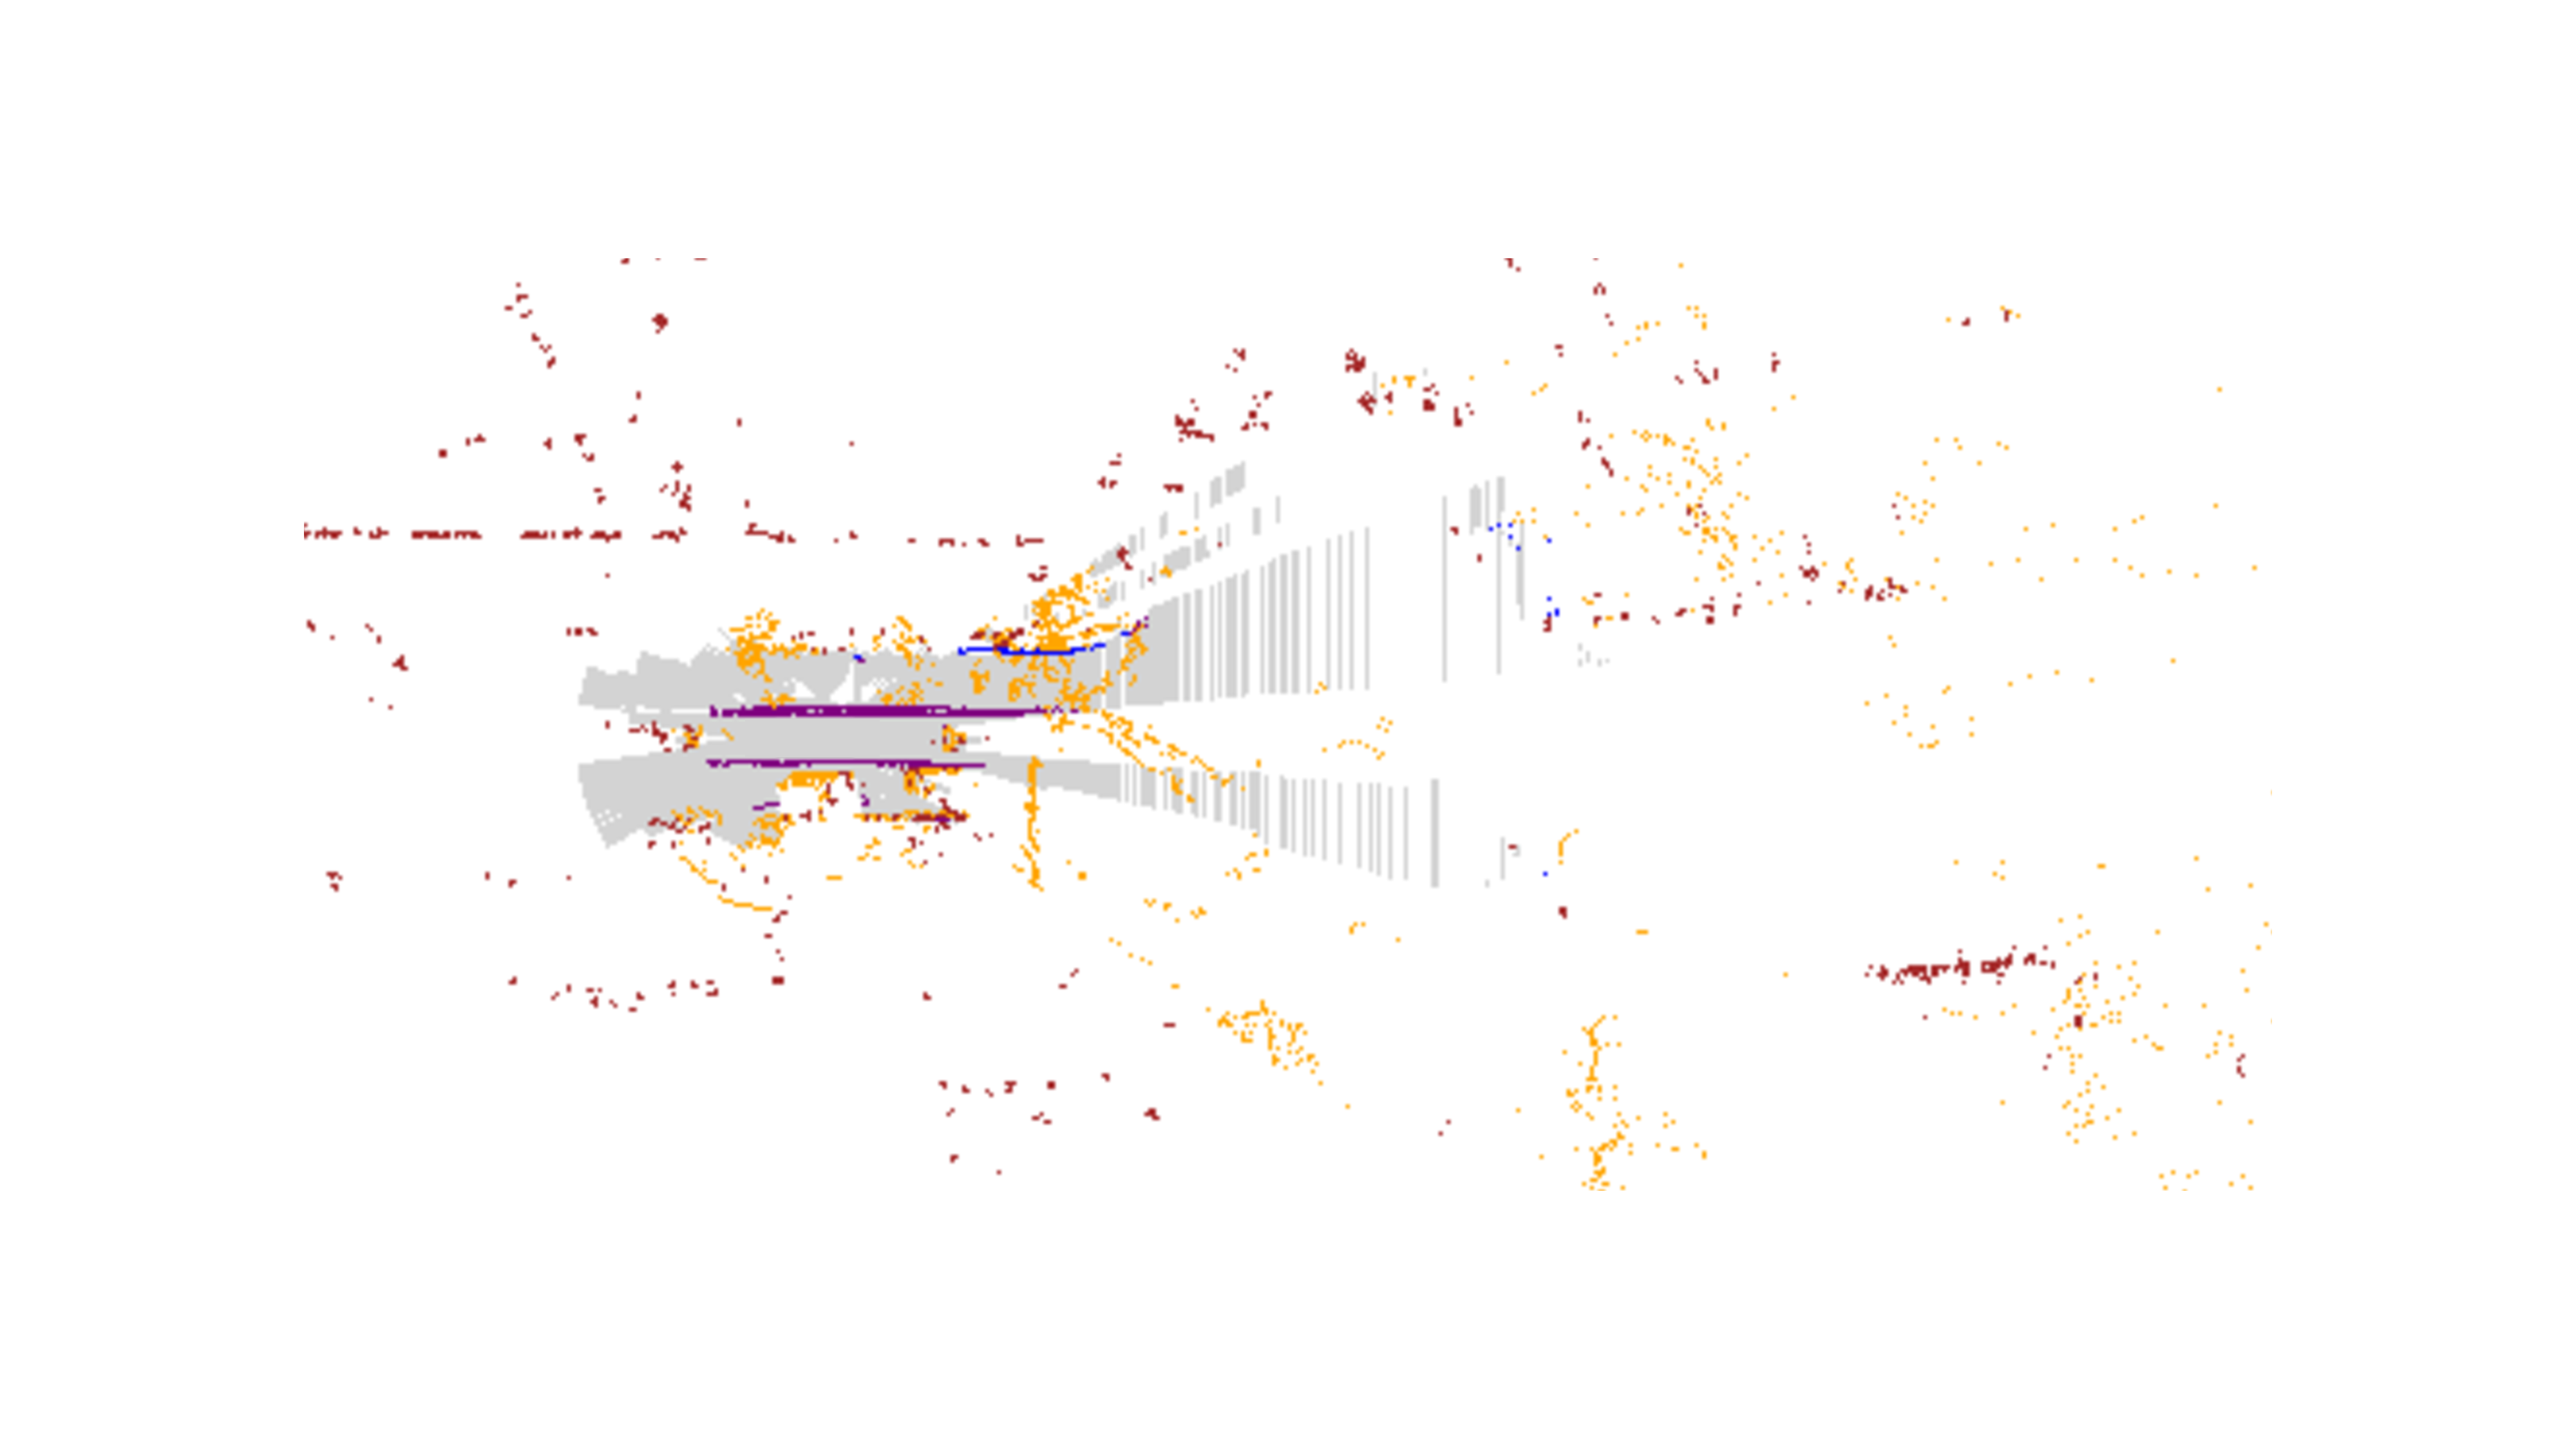
\includegraphics[width=0.85\linewidth]{LateX//figs/bevLoader.pdf}
        \caption{Layered Tensor Representation of Sensor Inputs}
        \label{fig:bev-loader}
    \end{figure}

    \item \textit{Ego Loader}: this component represents the ego vehicle within the same tensor used for other sensor data, specifically representation containing its ego-measures. A function is called to generate a rectangular outline representing the vehicle's physical dimensions. These dimensions correspond to the actual vehicle used to record the dataset sequences, ensuring accurate alignment in the scene. 
    The function takes as input the vehicle's specific coordinates, including key spatial points and orientations, particularly the heading angle, which defines the vehicle's facing direction relative to the map or environment frame. The resulting rectangular representation helps the network integrate the ego vehicle's precise location and orientation into the BEV tensor, serving as a reference point for other sensory data layers.
    \begin{figure}[H]
        \centering
        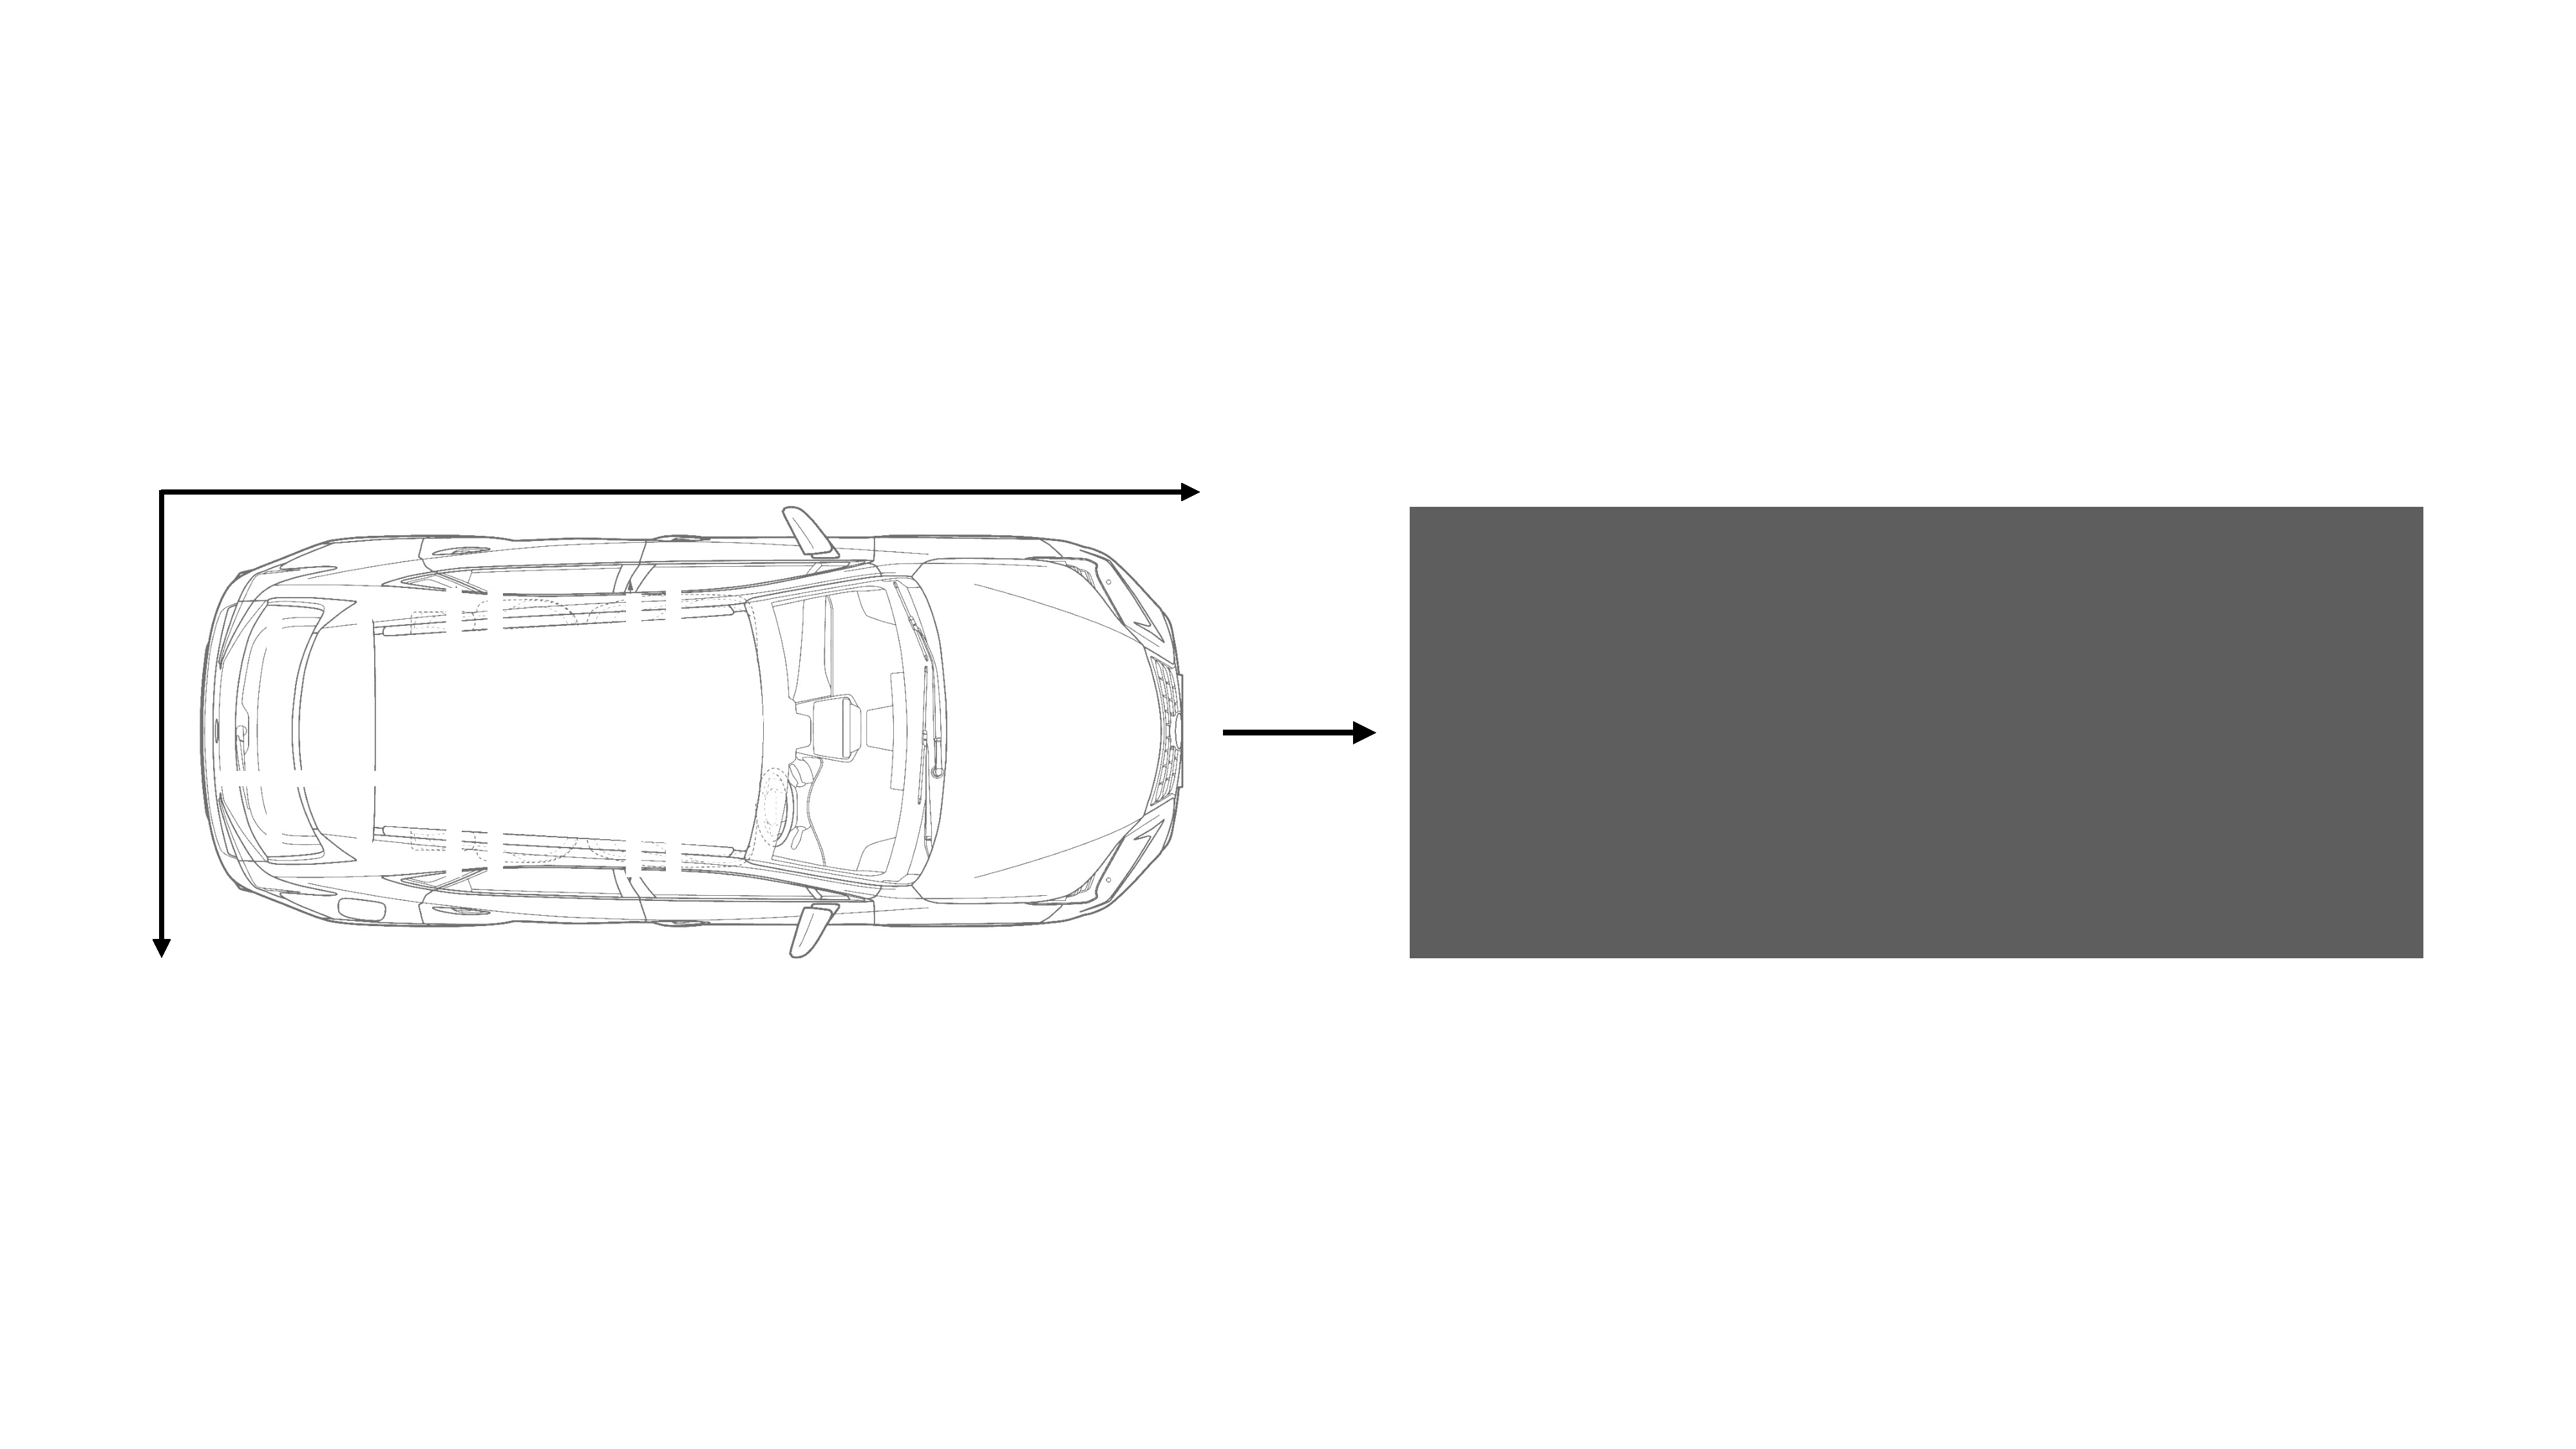
\includegraphics[width=0.75\linewidth]{LateX//figs/egoLoader.pdf}
        \caption{Tensor Representation of Ego Vehicle}
        \label{fig:ego-loader}
    \end{figure}

    \item \textit{Boundaries Loader}: this data-loader is responsible for semantic segmentation of the operational environment’s boundaries. This loader creates a tensor representing these boundaries, taking as input a dictionary containing HD map data of the relevant area. The reference area’s dimensions are configured in the settings file, which specifies the rectangular region around the vehicle’s position from which boundaries are extracted.
    Boundaries are downloaded from the HD map within a specified height and width limit around the vehicle's current location. This bounding box approach ensures that only the necessary map data is loaded, enhancing efficiency while focusing on the immediate environment.
    \begin{figure}[H]
        \centering
        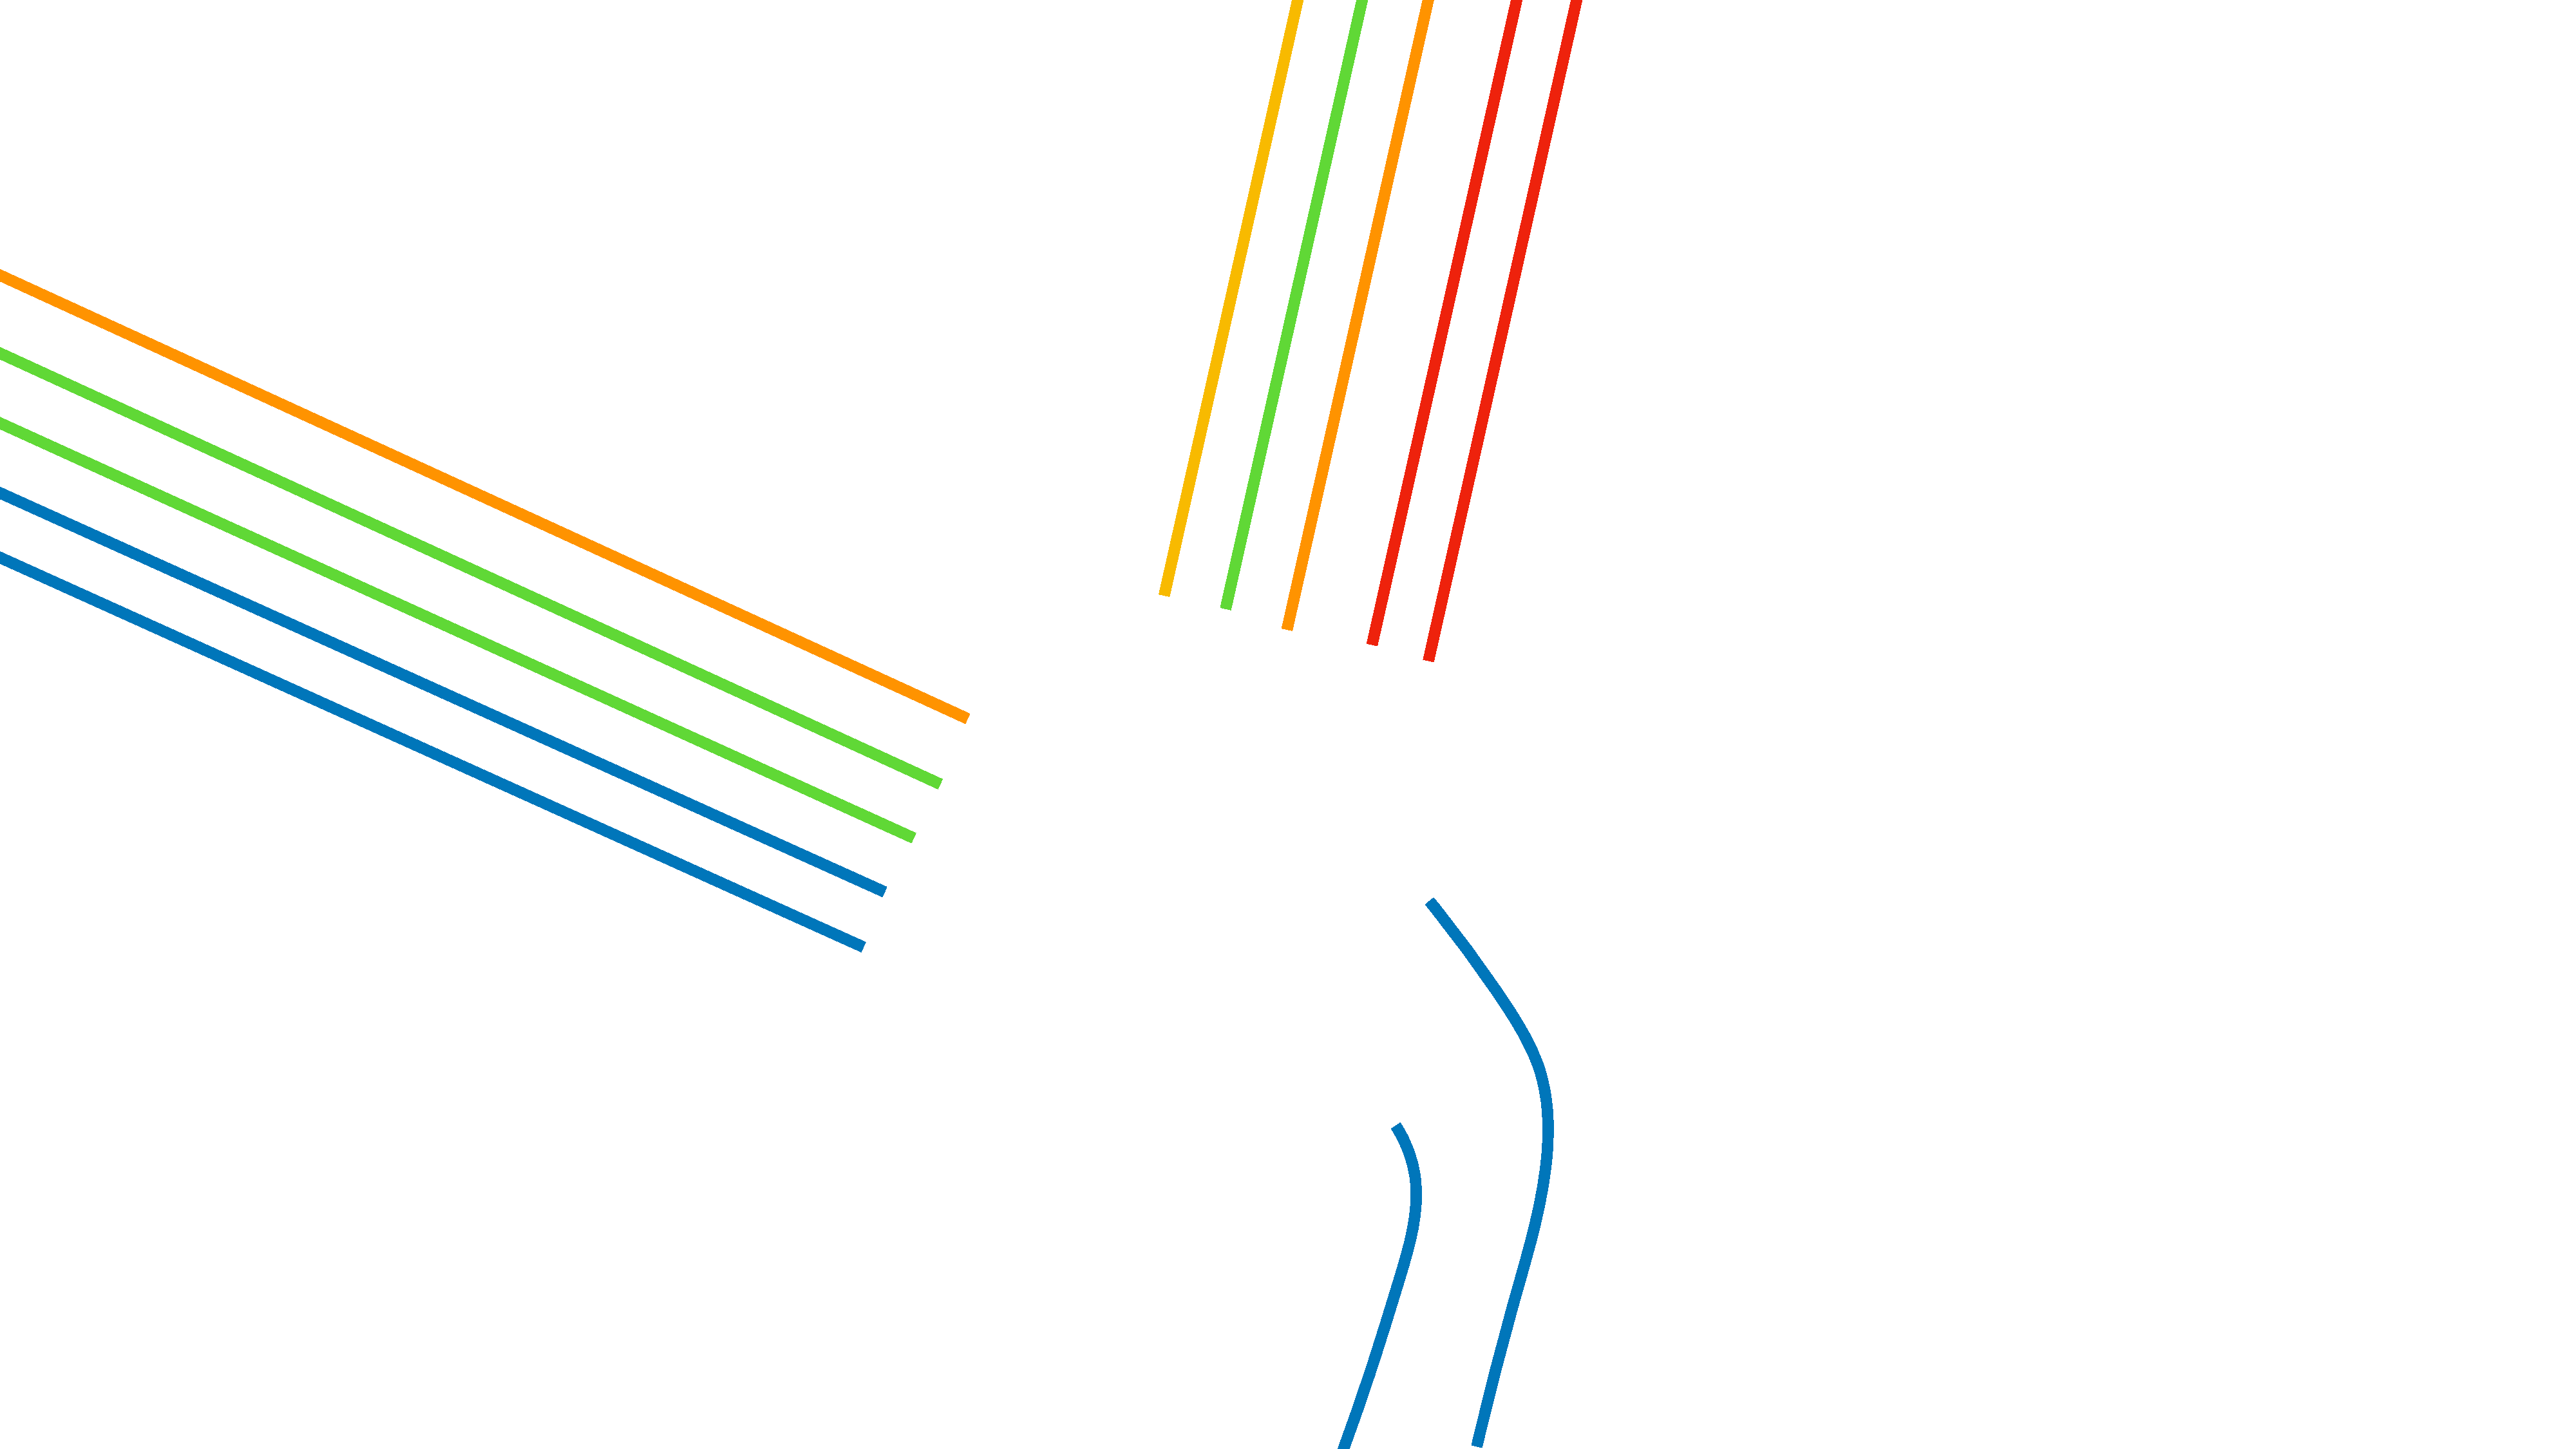
\includegraphics[width=0.75\linewidth]{LateX//figs/mappaHD.pdf}
        \caption{Boundaries on HD Map}
        \label{fig:hd-map-boundaries}
    \end{figure}
    In autonomous driving, \textit{boundaries} define the edges or limits of the vehicle's operational area. These include physical elements such as road edges, curbs, walls, or even virtual markers within a mapped area, all designed to constrain the vehicle’s movement within a safe and permissible space. Boundaries differ from lane markers: while lanes guide the vehicle along its intended travel path, boundaries prevent it from straying outside its permitted area or entering restricted zones. Essentially, boundaries provide containment for safe navigation, while lanes offer directional alignment within the road structure.
    The map data is represented with a fixed spatial resolution to ensure accurate alignment with the vehicle’s position. Specifically, each pixel corresponds to $25$ centimeters in the real world, providing a detailed, high-resolution representation suitable for tasks requiring precise localization. 
    To focus on the relevant area around the vehicle, the map is queried within a predefined spatial boundary. The queried map area extends from $-32$ meters to $96$ meters along the x-axis and from $-32$ meters to $32$ meters along the y-axis, effectively covering the area surrounding the vehicle’s operational zone.
    Additionally, the map compression settings help manage data density based on distance. Within a set proximity, the map’s resolution is maintained at a step of 5 meters per pixel in both x and y directions. Beyond specific distances (50 meters in x, 20 meters in y), compression is applied, reducing the map's data density to improve computational efficiency while retaining essential detail near the vehicle.
    This balance between map precision and computational efficiency ensures the network receives high-quality spatial data, which supports accurate and efficient map-based localization and alignment.
    Using OpenCV’s \texttt{draw\_polyline} function, boundaries are traced onto the tensor, with each boundary rendered as an anti-aliased line (of type \texttt{LINE\_AA}) with a thickness of 3 pixels. This line type provides smooth and visually clear boundary representations, ensuring that boundaries are accurately depicted in the tensor, as it can be seen in the Figure below.
    \begin{figure}[H]
        \centering
        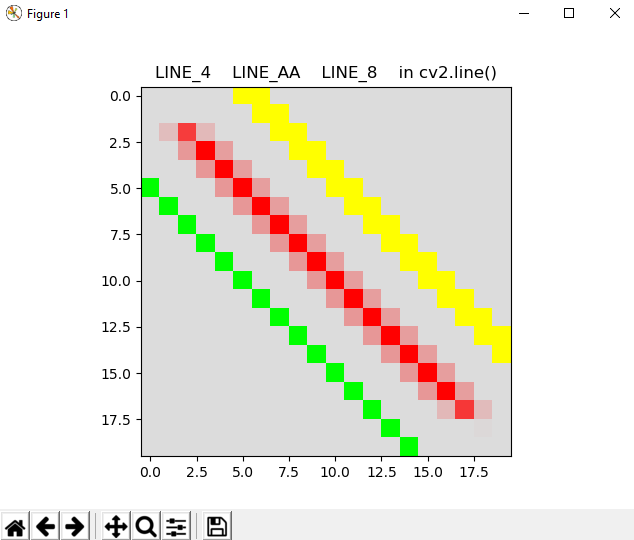
\includegraphics[width=0.5\linewidth]{LateX//figs/polyline.png}
        \caption{IMMAGINE DA SISTEMARE}
        \label{fig:enter-label}
    \end{figure}

    \item \textit{Texture Loader}: this loader is responsible for loading all images from the various cameras included in the sensor suite (as discussed in the relevant section). Each camera provides a unique view of the environment, capturing distinct visual information that the network can utilize for perception tasks.
    Historically, the term \textit{texture} was used in computer graphics to refer to images applied to 3D models or surfaces, giving them realistic visual details, such as color, pattern, and surface irregularities. 
    \begin{figure}[H]
        \centering
        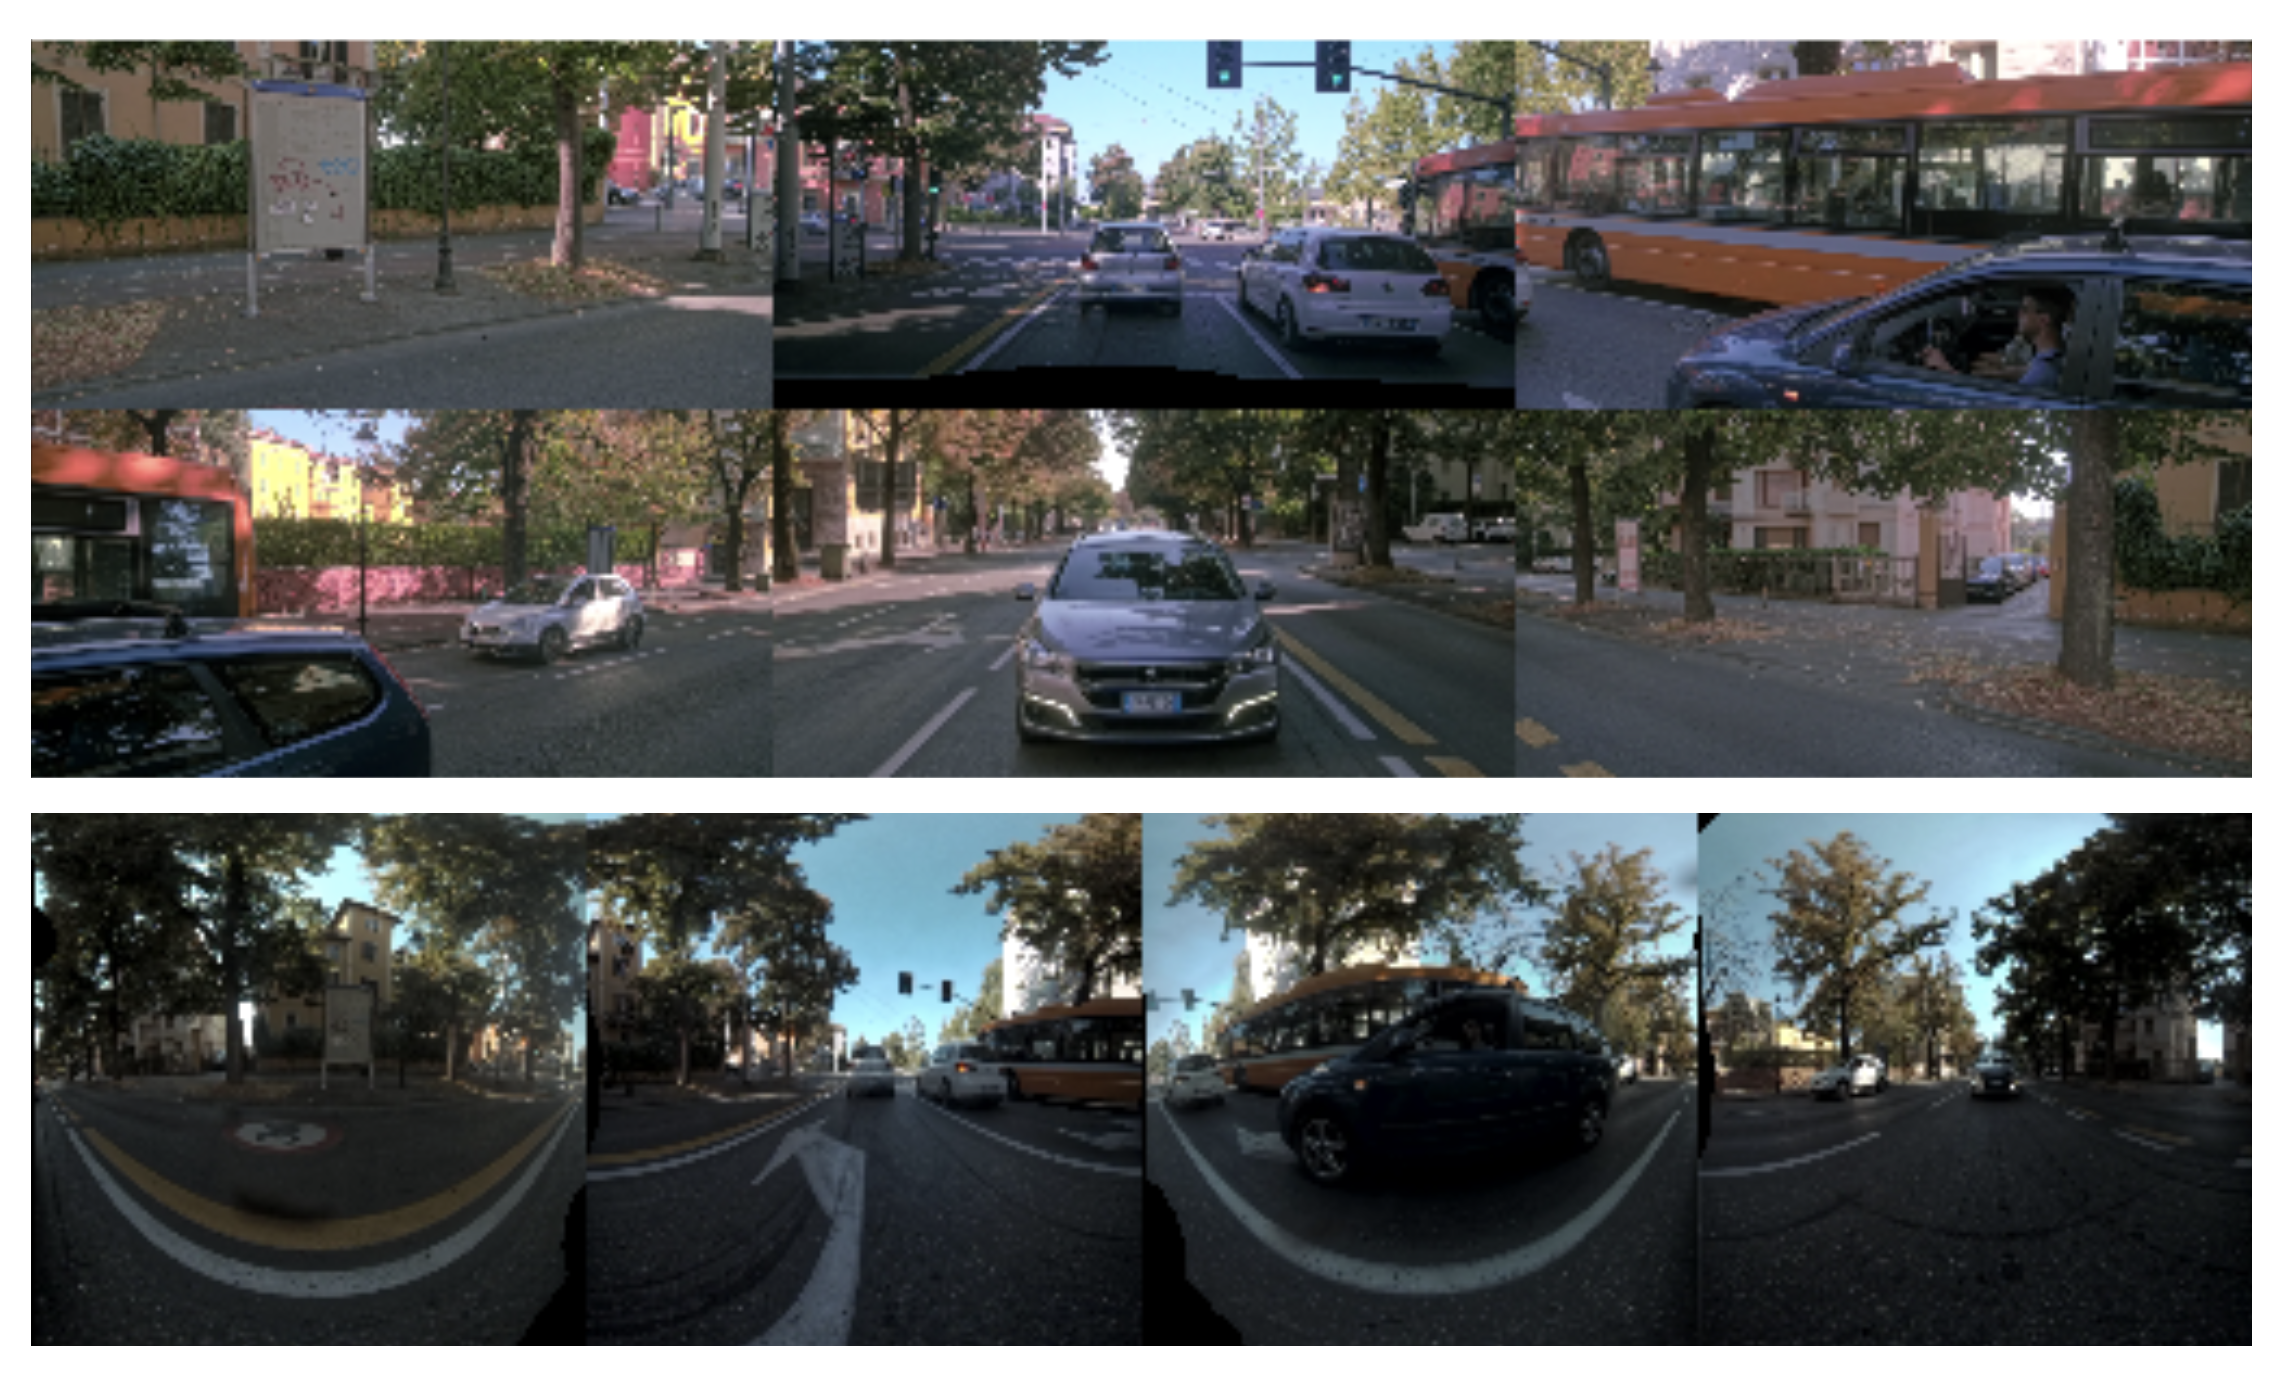
\includegraphics[width=0.95\linewidth]{LateX//figs/Screenshot 2024-09-27 at 12.00.55.png}
        \caption{Camera Textures: Images from Multiple Views}
        \label{fig:texture-loader}
    \end{figure}

    \item CamPosLoader

\end{itemize}

\subsection{Data Augmentation} 

Data augmentation is a technique used to artificially increase the diversity of training data by applying random transformations. This enhances the model’s ability to generalize to real-world variations not fully captured in the original dataset, making it more robust to unexpected changes in the input data \cite{MUMUNI2022100258}.

In this project, data augmentation is applied to simulate variations in the vehicle's position and orientation relative to the map. Using the optimized ground-truth position, known as \texttt{opt\_pose}, as the reference, augmentation introduces random rotations and shifts to mimic changes in the vehicle’s pose. This method accounts for slight discrepancies between the map alignment and the vehicle’s sensor data, preparing the model to handle similar disarrange during real-world application.

Specifically, the data augmentation involves:
\begin{itemize}
    \item Rotation: The map is randomly rotated within a range of -30 to 30 degrees to simulate orientation variations between the map and the vehicle.
    \item The map is shifted horizontally and vertically by up to 10\% of the image’s width and height, respectively, to account for minor lateral and vertical misalignments.
\end{itemize}

This augmentation strategy, applied during the training phase, helps the model generalize to various possible misalignments between the map and vehicle data, thereby improving robustness.

Directly using GNSS (Global Navigation Satellite System) data to align the map and vehicle pose can be problematic due to variability in GNSS accuracy. In some cases, GNSS data is highly accurate, providing near-perfect alignment with minimal adjustment effort. However, in other cases, GNSS data can be significantly inaccurate due to environmental factors like signal obstruction, leading to substantial misalignments. Relying solely on GNSS data would result in an imbalanced dataset, with some examples well-aligned and others poorly aligned, which could negatively impact the training process.

Using optimized positioning data that has been corrected through standard methods, a consistent and reliable ground-truth alignment is achieved, after which the previously described augmentation is applied, in order to get the most effective and well-balanced dataset possible.

In conclusion, all input loaders and data augmentation techniques have been described, detailing how each component contributes to the model's input preparation process. With these loaders and transformations in place, the network ultimately receives a well-structured and comprehensive input representation. This input integrates data from various sensors and includes augmented variations to ensure robustness, as illustrated in the figure below. The combined effect of these processes equips the network with diverse and realistic data, enhancing its ability to generalize in real-world applications.

\subsection{Target Loader}
The target loader is responsible for providing the target values that the network aims to predict. As previously described, these target values represent the transformations applied by the data augmentation block. Specifically, the network is trained to predict the roto-translation parameters: the translations along the three spatial axes and the rotation around the heading axis.

This loader prepares the ground-truth values for these transformations, giving the network a reference for learning to estimate spatial adjustments. In this context, the four values the network must predict include:
\begin{enumerate}
    \item Translation along the x-axis,
    \item Translation along the y-axis,
    \item Translation along the z-axis, 
    \item Rotation around the heading (yaw) axis.
\end{enumerate}
By learning these values, the network can effectively align the augmented data back to its original position, enhancing its robustness and accuracy in spatial localization.

\section{Dataset}
The dataset consists of multiple sequences recorded in various urban areas, capturing diverse driving conditions and environments. Each frame in these sequences includes not only the visual data but also synchronized information from all sensors mounted on the vehicle. This data packaging is managed by SuperDAG, a system designed by Vislab and Ambarella, which ensures synchronized data processing from the full perception suite.

All data is packaged into a \texttt{.bin} file format to optimize storage and facilitate efficient data handling. The dataset is collected from autonomous test vehicles equipped with varying sensor suites, typically including:
- Long-range cameras,
- Short-range cameras,
- Radars, and
- GPS/GNSS sensors.
\subsection{Sensor Suite}

\begin{figure}
    \centering
    \includegraphics[width=1\linewidth]{LateX/figs/sensor_suite2.pdf}
    \caption{Illustration of the Sensor Suite Configuration. Note: Two corrections are needed in this figure—first, the central rear radar should not be present in the BEV; second, the RR (Rear Right) label in the rear view is not centered.}
    \label{fig:sensor-suite}
\end{figure}

The long-range cameras can be utilized either as stereo cameras or mono cameras, depending on the type of test being conducted. In the specific sequences used for this project, data is sourced from six stereo cameras with a $120$-degree field of view. These cameras capture images at a resolution of $3840 \times 2160$ pixels and are used at a scale of $2$ (i.e., their dimensions are halved through pyramid scaling). This down-scaling facilitates faster inference operations by reducing computational load while retaining essential visual information.

Short-range cameras are positioned lower on the vehicle to enable a 360-degree reconstruction of the environment around the car. These cameras capture images at a resolution of $1920 \times 1080$ pixels and are used at full scale. Like the long-range cameras, they are stereo cameras but with a smaller baseline. This configuration allows for deterministic and traditional depth measurements of objects, making it easier to accurately position them within the world coordinates.

Pros of Using Stereo Cameras:
\begin{itemize}
    \item 3D Reconstruction: Stereo cameras enable the creation of 3D models and depth maps, providing a more comprehensive understanding of the scene by capturing spatial relationships between objects.
    \item Classification: The depth and location information from stereo images assist in classifying objects based on their three-dimensional positioning, enhancing object recognition capabilities.
\end{itemize}

Cons of Using Stereo Cameras:
\begin{itemize}
    \item Cost: Implementing stereo cameras requires double the hardware compared to mono cameras, and they demand powerful processing units to handle the increased data volume.
    \item Calibration Maintenance: Regular calibration is necessary to ensure accurate depth perception and alignment between the cameras. Any misalignment can lead to errors in depth estimation.
    \item Mechanical Challenges: Higher sensor resolutions in stereo setups can introduce mechanical complexities, such as the need for auto-calibration mechanisms to maintain alignment over time.
\end{itemize}

Another crucial set of sensors are radars, which offer different advantages and disadvantages compared to stereo cameras. Radars are less dependent on external lighting conditions, allowing for reliable object detection in various weather and lighting scenarios.

**Radio Detecting and Ranging (RADAR)** is a system used to detect the distance, angle, and speed of objects relative to the sensor. It operates by emitting radio or microwave signals using an array of antennas and capturing the signals that bounce back from objects in the environment. By processing these received signals, the system can extract the position, angle, and speed of targets.

The signal frequency used by radar systems can range from 1 to 110 GHz. Air traffic control applications require higher precision and thus use higher frequencies, while automotive applications typically use frequencies between 40 and 77 GHz. The time of flight for radar signals is approximately 6 microseconds per kilometer, allowing for rapid distance calculations. A frequency shift in the returned signal, known as the Doppler effect, is related to the speed of the target object.

Radar systems often employ a chirp or sweep signal—where the frequency increases or decreases over time—to improve the separation of targets and enhance resolution. Radars have been a consolidated technology in automotive applications for over 30 years, offering reliable performance even in adverse weather conditions. However, they may face challenges in detecting two closely spaced objects due to separation limitations.

Types of Automotive Radars:
\begin{itemize}
    \item Long-Range Radars: Capable of detecting objects up to 300 meters away, suitable for Adaptive Cruise Control (ACC) and highway driving scenarios.
    \item Medium-Range Radars: With a range of about 100 meters, these are effective for detecting cross traffic, aiding in lane changes, and merging maneuvers.
    \item Short-Range Radars: Effective up to 30 meters, ideal for low-speed maneuvers such as parking and navigating in tight spaces.
\end{itemize}

On the test vehicle, multiple radars are installed, including one long-range radar positioned at the front of the vehicle and several medium-range radars strategically placed to cover the surrounding environment.

At the conclusion of the dataset description, it is pertinent to highlight the specific areas of the city where the recorded sequences were collected. The data was gathered in various locations around Parma, including Via Langhirano, the train station area, and the Parma Fairgrounds. These sequences comprise a total of [insert total frame count] frames, which were divided into training and validation sets to facilitate the model's development and evaluation.

During the project's development, two different dataset splits were utilized. Initially, only sequences from a specific area were used to reduce data volume and focus on refining the model's structure and functionality. This approach allowed for rapid iteration and debugging without the complexity of a large, diverse dataset. Once the foundational methodology was established and the optimal workflow was determined, the dataset was expanded to include all available recorded sequences. This expansion introduced greater diversity and complexity, enhancing the model's ability to generalize across different environments.

The sequences are varied, captured under diverse weather conditions and traffic scenarios, including both well-lit days and nighttime recordings with varying illumination levels. Some sequences were recorded in adverse weather conditions, contributing to the dataset's robustness. Additionally, certain sequences lack data from some cameras (referred to as "missing modalities"). This variation is advantageous, as it trains the model to be robust against different sensor suite configurations and to handle scenarios where some sensor data may be unavailable.

\section{Methodology}

This section outlines the methodology employed to solve the task. After defining all the inputs and targets for the network and deserializing the required data, it is essential to describe the tools and frameworks utilized in the project. The model's detailed description and the various attempts made will be presented in the subsequent section.

The entire code-base was developed in Python, chosen for its compatibility with PyTorch, the primary tool used for the neural network implementation. **PyTorch** is an open-source machine learning library developed by Facebook's AI Research lab (FAIR) in 2016. It provides a flexible platform for deep learning research and production, emphasizing dynamic computation graphs and efficient tensor computations. PyTorch's use of tensors—multi-dimensional arrays similar to NumPy arrays but with support for GPU acceleration—makes it well-suited for the computational demands of deep learning tasks.

For training the neural network, \textit{CUDA} (Compute Unified Device Architecture) was employed to leverage GPU acceleration. CUDA is a parallel computing platform and programming model developed by NVIDIA, enabling dramatic increases in computing performance by harnessing the power of graphics processing units (GPUs). By utilizing CUDA, the code can perform parallel computations efficiently, significantly reducing training time and improving performance.

The training phase was conducted on a dedicated server equipped with three NVIDIA Tesla V100 GPUs, each with 32 GB of memory, 256 GB of RAM, and a 64-core processor. Despite the availability of multiple GPUs, most of the training utilized a single GPU due to concurrent tasks that needed to be managed simultaneously. This setup provided the necessary computational resources to handle the intensive processing requirements of training deep neural networks.
